\documentclass [xcolor=svgnames, t] {beamer} 
\usepackage[utf8]{inputenc}
\usepackage{booktabs, comment} 
\usepackage[absolute, overlay]{textpos} 
\usepackage{pgfpages}
\usepackage[font=footnotesize]{caption}
\useoutertheme{infolines} 
\graphicspath{{D:/Project file/Project file/Presentation - V2/images/}}

\definecolor{brownbrown}{RGB}{56, 28, 0}
\definecolor{brownred}{RGB}{255,255,0}

\setbeamercolor{title in head/foot}{bg=brownred, fg=brownbrown}
\setbeamercolor{author in head/foot}{bg=myuniversity}
\setbeamertemplate{page number in head/foot}{}
\usepackage{csquotes}


\usepackage{amsmath}
\usepackage[makeroom]{cancel}
\usepackage[utf8]{inputenc}
\usepackage[retainorgcmds]{IEEEtrantools}
\usepackage{graphicx}
\usepackage{verbatim}
\usepackage{array}
\usepackage{slashbox}
\usepackage{multirow}
\usepackage{setspace}
\usepackage[para]{threeparttable}
\usepackage[english]{babel}
\usepackage{ragged2e}
\usepackage{etoolbox}
%\usepackage{footnote}
\apptocmd{\frame}{}{\justifying}{} % Allow optional arguments after frame.
\usepackage{sansmathaccent}
\pdfmapfile{+sansmathaccent.map}
\usepackage{float}
\usepackage[caption = false]{subfig}
%\usepackage[demo]{graphicx}
\usepackage{tikz}
\usetikzlibrary{matrix,shapes,arrows,positioning,chains,decorations.markings,calc}
\usepackage{verbatim}
\graphicspath{{D:/Thesis Presentation/images/}}
\usetheme{Madrid}
\definecolor{myuniversity}{RGB}{0,100,0}
\usecolortheme[named=myuniversity]{structure}
\usepackage{tikz}
\usepackage{float}
\usepackage{subfig}
\usepackage{caption}
\captionsetup[figure]{font=scriptsize}
\beamertemplatenavigationsymbolsempty
%\setbeamertemplate{footline}[frame number]

\title[PG THESIS]{}
\subtitle{\large EVALUATION OF CATASTROPHIC INDICATORS FOR POWER SYSTEM STABILITY ASSESSMENT}
\author[Subha Biswal] % (optional, for multiple authors)
{\small by \\ \large\textbf{Subha Biswal} \\ \small Power System Engineering \\ Dual Degree \\ (Reg. No. 1704050016)}
 
\institute[EE] % (optional)
{
\small Under the guidance of\\
\large \textbf{Dr. Rajat Kanti Samal}
%  \and
%  \inst{2}%
%  Faculty of Chemistry\\
%  Very Famous University
}

\logo{
\includegraphics[height=1 cm]{VSSUTLogo.png}}
 
\date[May 2022] % (optional)
{
Department of Electrical Engineering\\
Veer Surendra Sai University of Technology\\
Burla, Odisha – 768018
}


\addtobeamertemplate{navigation symbols}{}{%
    \usebeamerfont{footline}%
    \usebeamercolor[fg]{footline}%
    \hspace{1em}%
    \insertframenumber/\inserttotalframenumber
}

\begin{document}
\begin{frame}
\maketitle
\end{frame}


%%%%%%%%%%%%%%%%%%%%%%%%%%%%
\logo{
\includegraphics[height=1.0cm]{VSSUTLogo.png}~%
}
%%%%%%%%%%%%%%%%%%%%%%%%%%





\begin{frame}{Contents}
\begin{itemize}
\item Objectives
\item Organisation of Catastrophic Indicators
\item Solution Methodology
\item Results and Discussion
\item Conclusion
\item Future Scope
\item References
\end{itemize}
\end{frame}

\begin{frame}{Objectives}
\begin{itemize}
\item To use MAT-POWER toolbox along with MATTRANS software to perform Transient Stability Analysis.
\item To prepare an algorithm and codes for Catastrophic Indicators for Power System Stability Assessment for Simulated PMU Data.
\item To obtain the results of indicators for simple transient stability analysis on IEEE 10 Bus and 145 Bus System
\end{itemize}
\end{frame}

\begin{frame}{Catastrophic Indicators}
\textbf{1. Indicator Based on Coherency:}
\begin{itemize}
\item Coherency is the measure of the closeness of all generator rotor angles after fault-clearing (or closeness to the center of inertia COI).
\item For example if the angles of all generators in Case A are closer to the COI after fault-clearing than in Case B, Case A is more coherent than Case B.
\item The Performance Index is calculated as the maximum difference of maximum and minimum angle for all generators in some short period (say, 0.5 second) after fault clearing.
\item $Performance \; Index = max\big(\theta_i(t)\big)-min\big(\theta_i(t)\big)$ 
\end{itemize}
\end{frame}

\begin{frame}{Catastrophic Indicators (cont.)}
\textbf{2. Indicator Based on Transient Energy Conversion:}
\begin{itemize}
\item Transient energy includes kinetic energy and potential energy.
\item The transient kinetic energy is mainly related to the speed of generators. The transient potential energy includes three parts: position energy of all rotors relative to the COI, magnetic energy, and dissipation energy.
\item If the system has enough potential energy capability, then the excess kinetic energy injected into the system can be “absorbed”, and the system will not lose synchronism, and reach a new stable equilibrium point.
\item $Performance \; Index = max\big(V_{ke}(t)\big) - min\big(V_{pe}(t)\big)$
\end{itemize}
\end{frame}

\begin{frame}{Catastrophic Indicators (cont.)}
\textbf{3. Indicator Based on Dot Products-  Contingency Severity Assessment (CSA):}
\begin{itemize}
\item A dot product. is defined for detecting the exit point in the Transient Energy Function method. 
\item AThe exit point is characterized by the first maximum of rotor angle deviation from COI with respect to the post-fault network. 
\item It is computed by the dot product of the fault-on rotor angle mismatch vector and the fault-on speed vector.
\item $CSA(t) = \sum_{i=1}^{N_{area}} V_i(t) = \sum_{i=1}^{N_{area}} \omega_i(t)[\delta_i(t) - \delta_i(0^+)]$
\item $Performance \; Index = max\big(CSA(t)\big) - min\big(CSA(t)\big)$
\end{itemize}
\end{frame}

\begin{frame}{Catastrophic Indicators (cont.)}
\textbf{4. Indicator Based on Wide Area Severity Index (WASI):}
\begin{itemize}
\item In a largely interconnected network, the power-transfer level increases, so to capture the fault severity of the area WASI indicator is defined.
\item The WASI is defined as the logarithm of power spectral density (PSD) of the CSA index.
\item At high power transfers, the signal energy exhibits an exponential increase, which can be captured through a log-linear relationship with power transfer.
\item Therefore, the indicator includes logarithmic aspect, which makes the indicator more sensitive when it needs.
\item $WAST(T) = log(max_{t \; \in \; [0^+,T]}(max_i(PSD(V_i(t)))))$
\item $Performance \; Index = max\big(WASI(t)\big) - min\big(WASI(t)\big)$
\end{itemize}
\end{frame}

\begin{frame}{Catastrophic Indicators (cont.)}
\textbf{5. Indicator Based on Inter-area Stability Prediction Index (ISPI):}
\begin{itemize}
\item It works on the basis of 2 components voltage-magnitude change (reduction) and the phase-angle movement (separation). 
\item This index can be an alternative to the aforementioned WASI, which is defined in the frequency domain.
\item considerable feature of this index is its fast and easy calculation from synchronously measured voltage without system modelling and simulation and without dependency on network size.
\item It calculates the percentage change in voltage magnitude and its rate of change and angle deviation from center of inertia (COI) and also its rate of change of each coherent area.
\end{itemize}
\end{frame}

\begin{frame}
\begin{itemize}
\item When these parameters change below a pre-specified threshold during system swings, an alert is done to prevent the system operator or to activate a control action.
\item The level of ISPI is obtained between 100\%, where
\begin{itemize}
\item Less than 33\% - Normal State
\item 33\% to 66\% - Alert State
\item More than 66\% - Alarm State
\end{itemize}
\item $ISPI = 1-(1-P\Delta V).(1-PV').(1-P\Delta d \delta gc).(1-Pd \delta gc')$
\end{itemize}
\begin{figure}[H]
	 \centering
	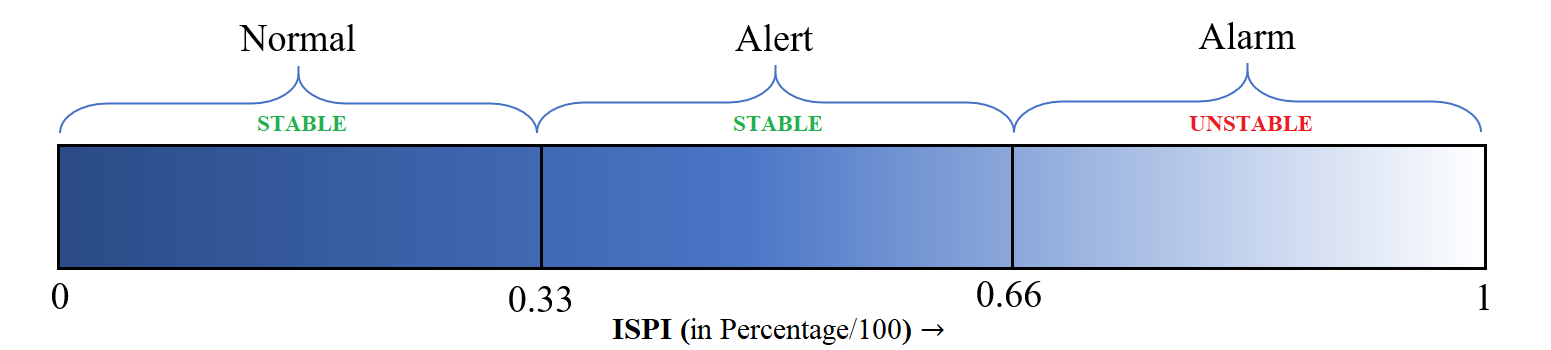
\includegraphics[width=10 cm]{ISPI Categories.png}
	\caption{Stability Prediction Index Categories}
	\label{ISPI Categories}
\end{figure}
\end{frame}

\begin{frame}{Solution Methodology Flowchart}
\begin{figure}[H]
	 \centering
	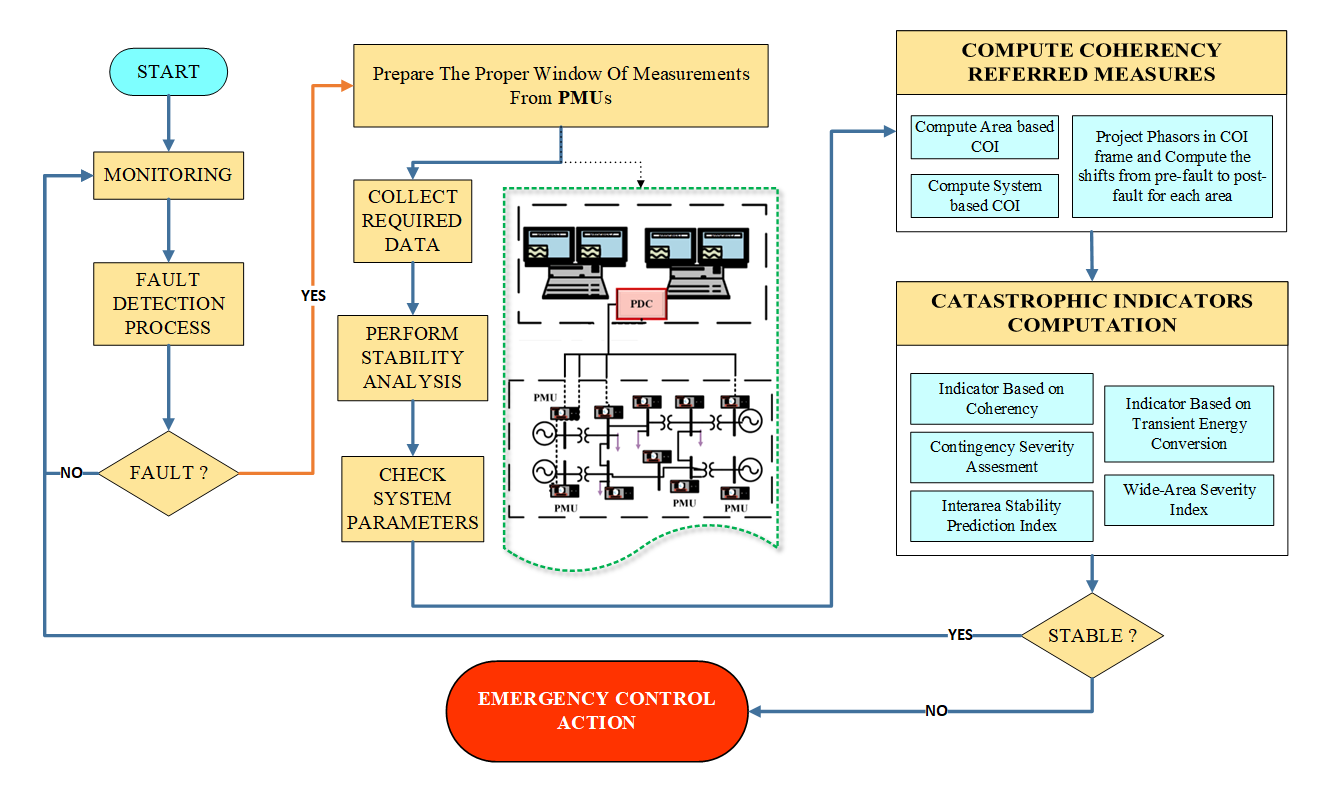
\includegraphics[width=12 cm]{Flowchart1.png}
	
\end{figure}
\end{frame}

\begin{frame}{MATTRANS Tool Box}
\begin{itemize}
\justifying
\item MATTRANS is a free and open-source programme package of MATLAB(R)/Simulink (M-files and .mdl files) for performing transient fault analysis, developed in 2008 by G. Ravikumar. 
\item The MATTRANS syntax for using it is \textbf{runts(case\# , case\# dd);} which needs two input files in .m format: 1) network steady-state data and 2) network dynamic data. The network steady-state data is used from MATPOWER, whereas the network dynamic data includes generator machine parameters, exciter parameters, turbine parameters, and power system stabilizing parameters.  
\item All these dynamic data are taken from the execution of base simulation model \textbf{transientStability.mdl}, which includes various sub models such as Turbine System, Excitation system, Power System Stabilizer Model, Static Loads And there system parameter outputs.
\end{itemize}
\end{frame}

\begin{frame}
	\frametitle{Transient Stability Model}
	\begin{itemize} \justifying 
	\item It is the base model which include various sub models to check for Transient Stability of a system, Main sub models includes Generators, Turbine System, Excitation system, Power System Stability Model, Static Loads and its outputs.
	\end{itemize}
	\begin{figure}
	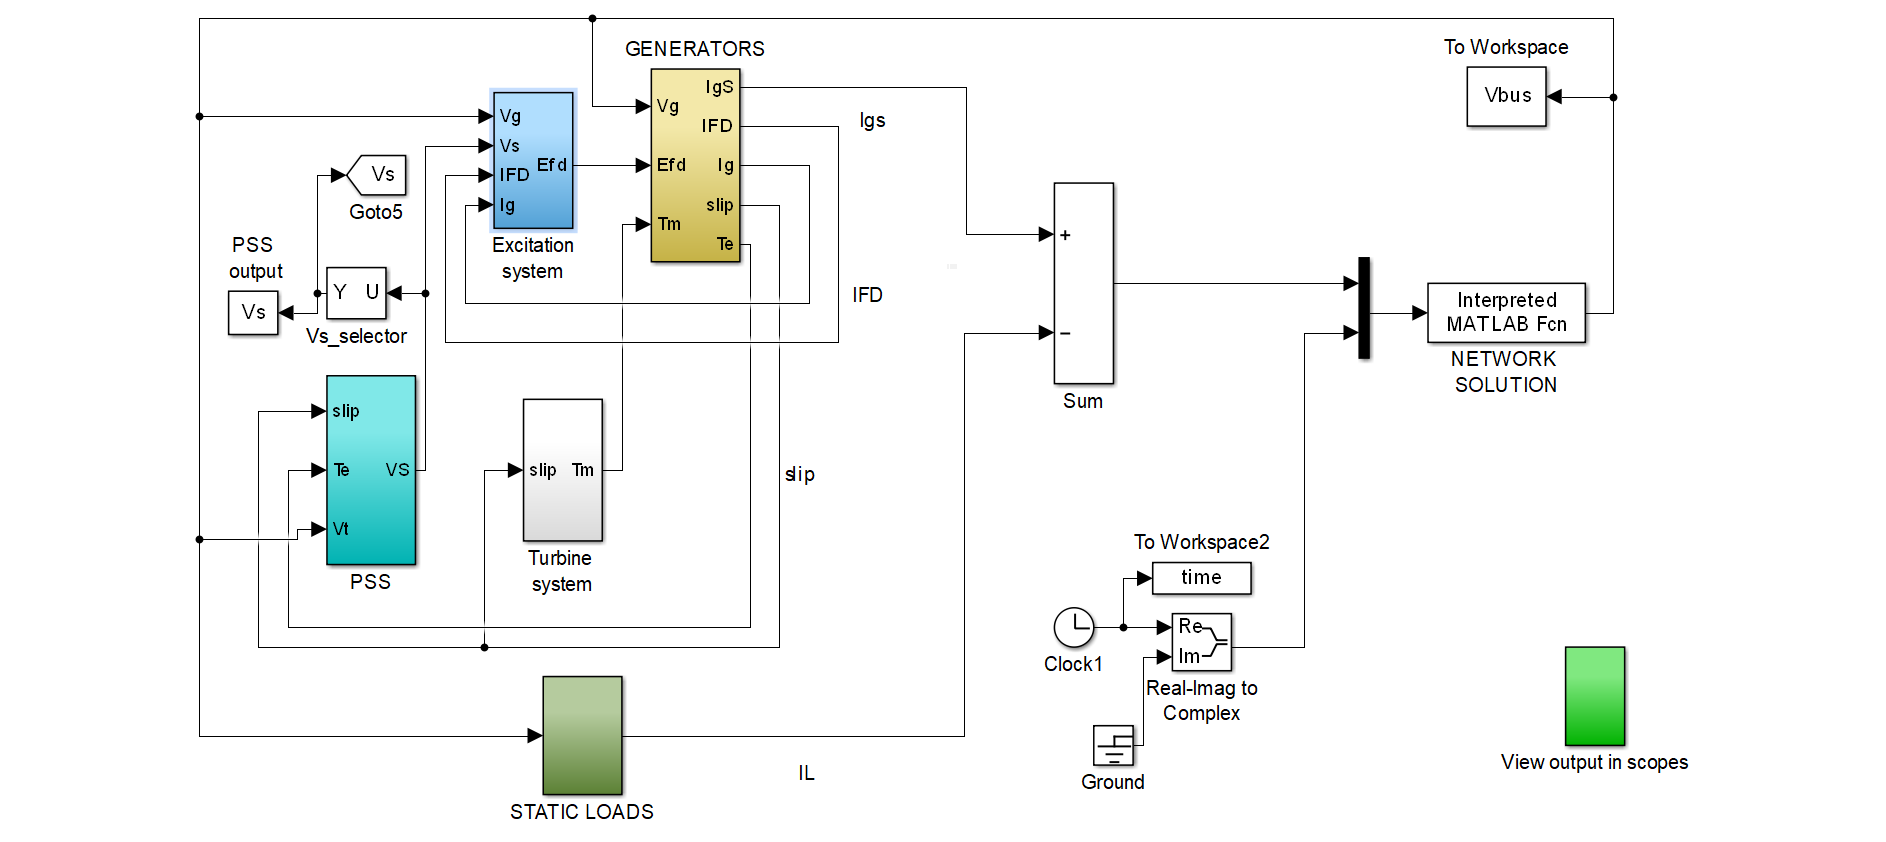
\includegraphics[scale=0.3]{Transient Stability}
	%\caption{Add your own figures before compiling}
	%\label{some example}
	\end{figure}
	\end{frame} 
	
	\begin{frame}
	\frametitle{Excitation System Model}
	\begin{itemize} \justifying 
	\item This is an excitation system created to do the work of an generator exciter, it takes input of Vg, Vs, IFD and Ig and with the help of different exciter system it  produces the Excitation voltage(EFD) and passes to the generator.
	\end{itemize}
	\begin{figure}
	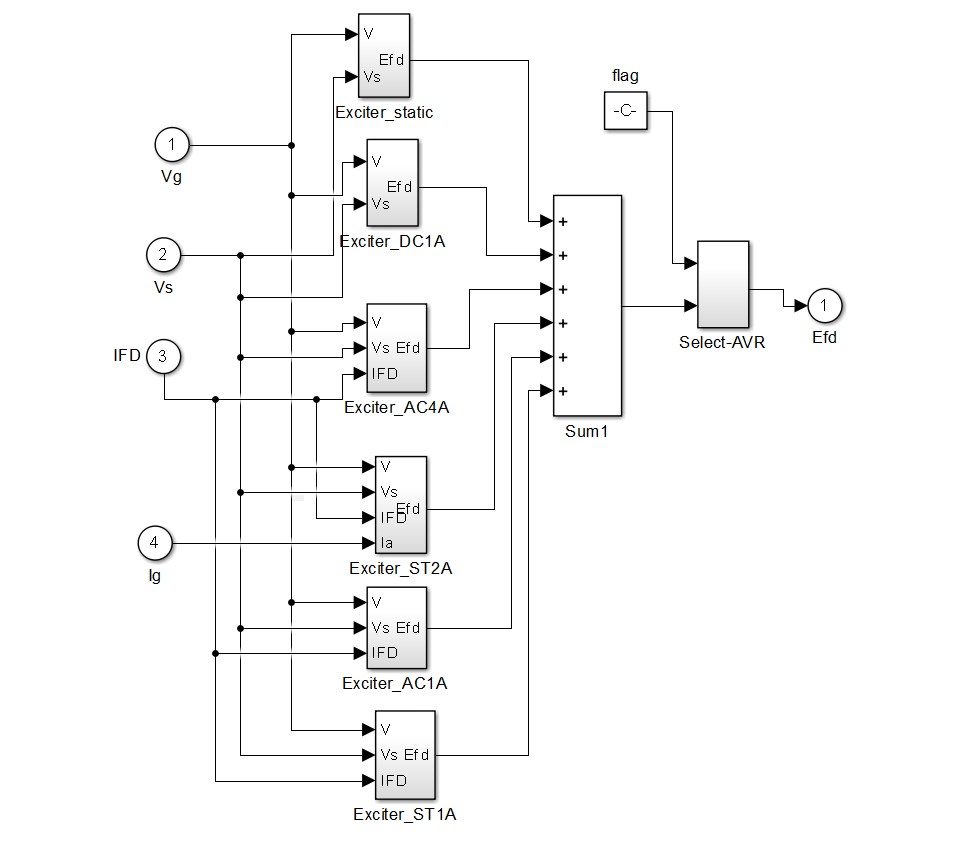
\includegraphics[scale=0.3]{Excitation Model}
	%\caption{Add your own figures before compiling}
	%\label{some example}
	\end{figure}
	\end{frame} 
	
	\begin{frame}
	\frametitle{Generator Model}
	\begin{itemize} \justifying 
	\item It is the Generator Model created to do the work of a normal generator (Electric machine) and along with calculating its parameters like torque, angle deviation, field current, saliency etc..
	\end{itemize}
	\begin{figure}
	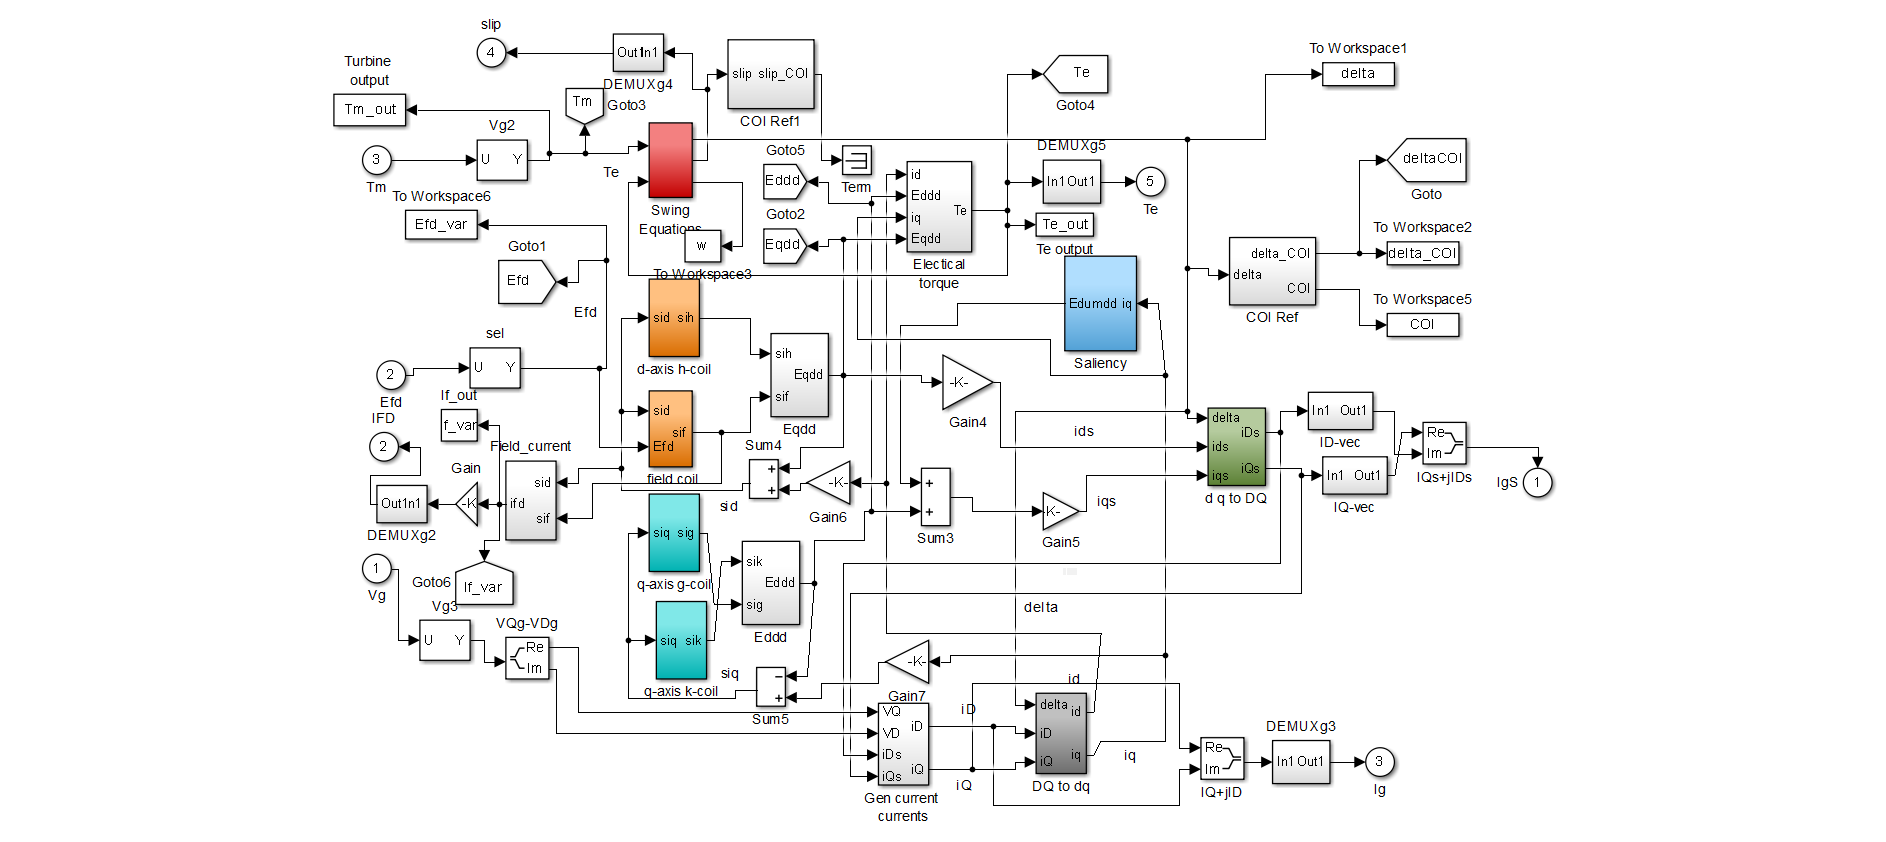
\includegraphics[scale=0.3]{Generators}
	%\caption{Add your own figures before compiling}
	%\label{some example}
	\end{figure}
	\end{frame} 
	
	\begin{frame}
	\frametitle{Power System Stabilizing Model}
	\begin{itemize} \justifying 
	\item It is created to give feedback to the excitation system according to the deviation of generator from the system parameters. It checks the generator slip and torque and bus voltage and by using four functions (Slip Signal, Power Input, Frequency Input and DelP\_Omega) it gives the feedback voltage.
	\end{itemize}
	\begin{figure}
	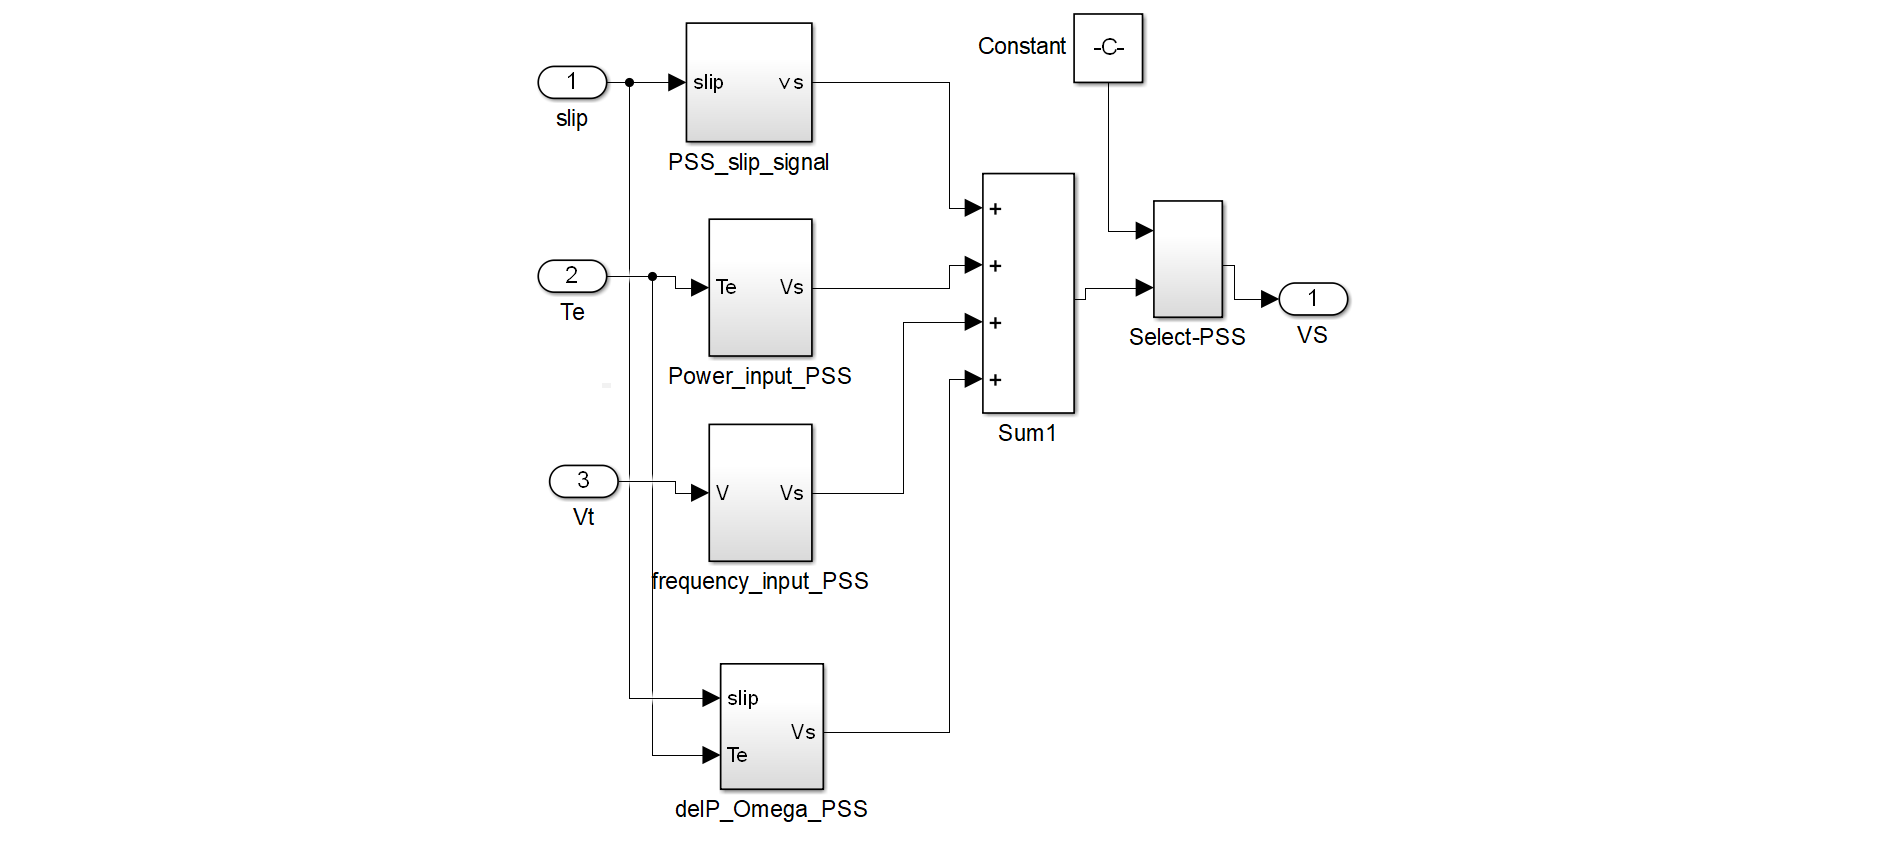
\includegraphics[scale=0.3]{PSS}
	%\caption{Add your own figures before compiling}
	%\label{some example}
	\end{figure}
	\end{frame} 
	
	\begin{frame}
	\frametitle{Static Loads Model}
	\begin{itemize} \justifying 
	\item This simulation model is prepared to create a load system which uses active and reactive part to calculate the consumption by the load with the help of various mathematical formulas and gives the current output to the system to calculate power consumption.  
	\end{itemize}
	\begin{figure}
	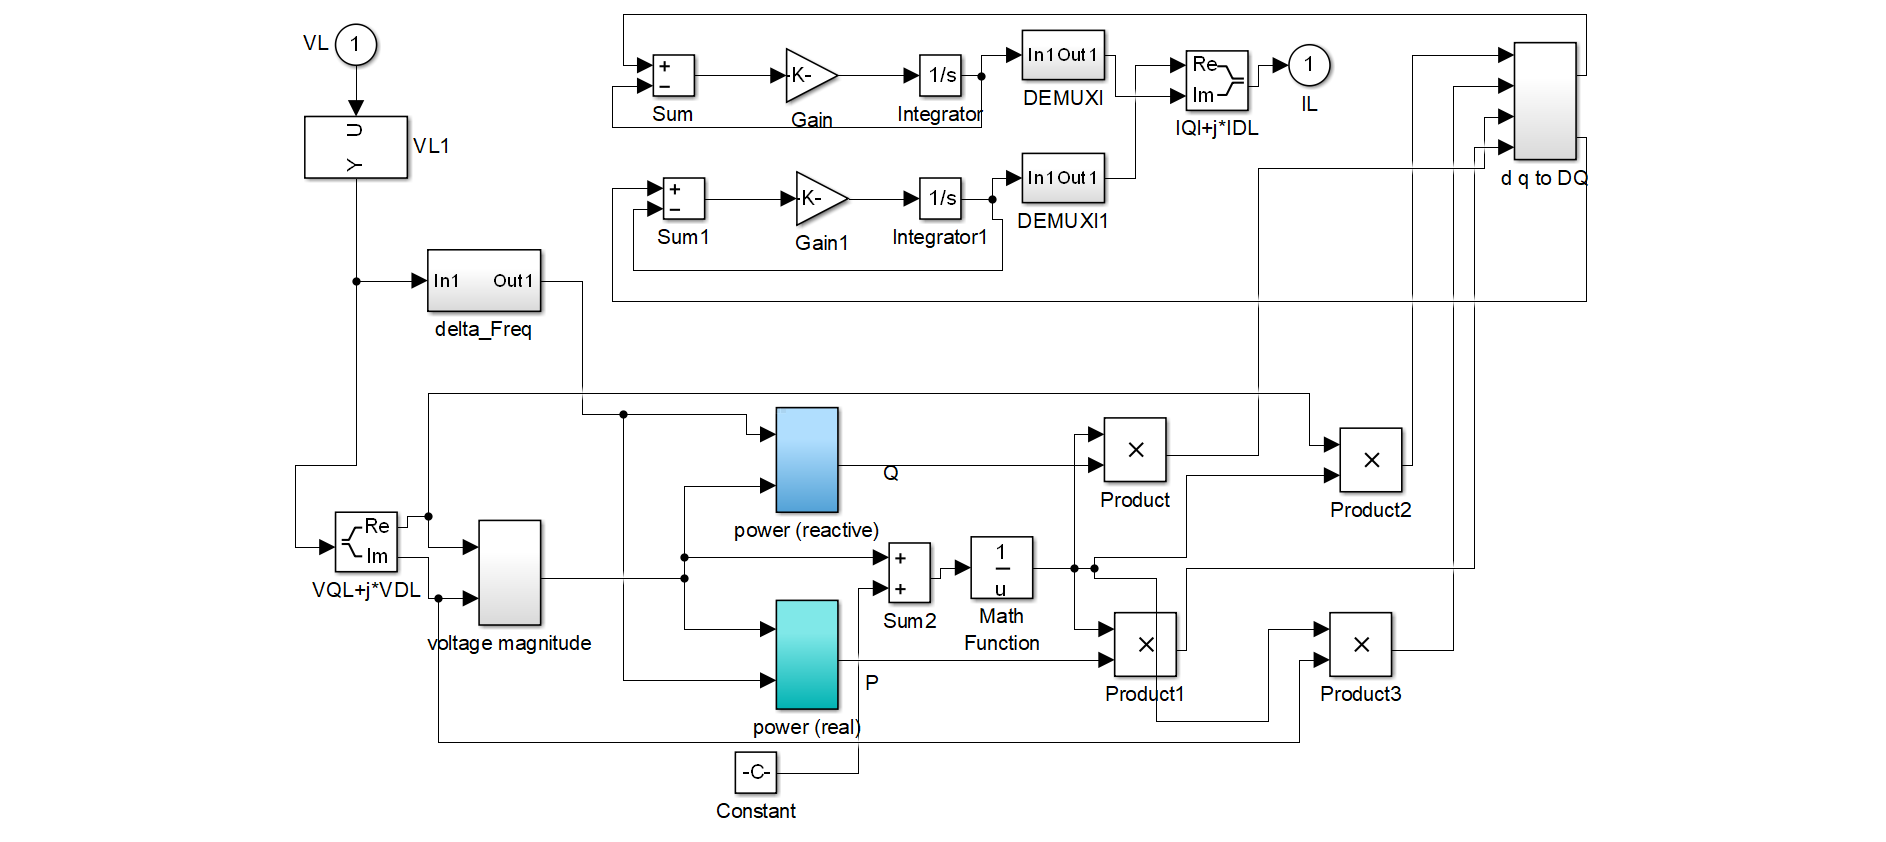
\includegraphics[scale=0.3]{Static Loads}
	%\caption{Add your own figures before compiling}
	%\label{some example}
	\end{figure}
	\end{frame}
	
	\begin{frame}
	\frametitle{Turbine System Model}
	\begin{itemize} \justifying 
	\item Different Turbine Systems are included such as Speed Governor Hydro Turbine, Speed Governor Reheat Steam turbine and Non Reheat Steam turbine to add Turbine parameters to check system variance in case of real time use.
	\end{itemize}
	\begin{figure}
	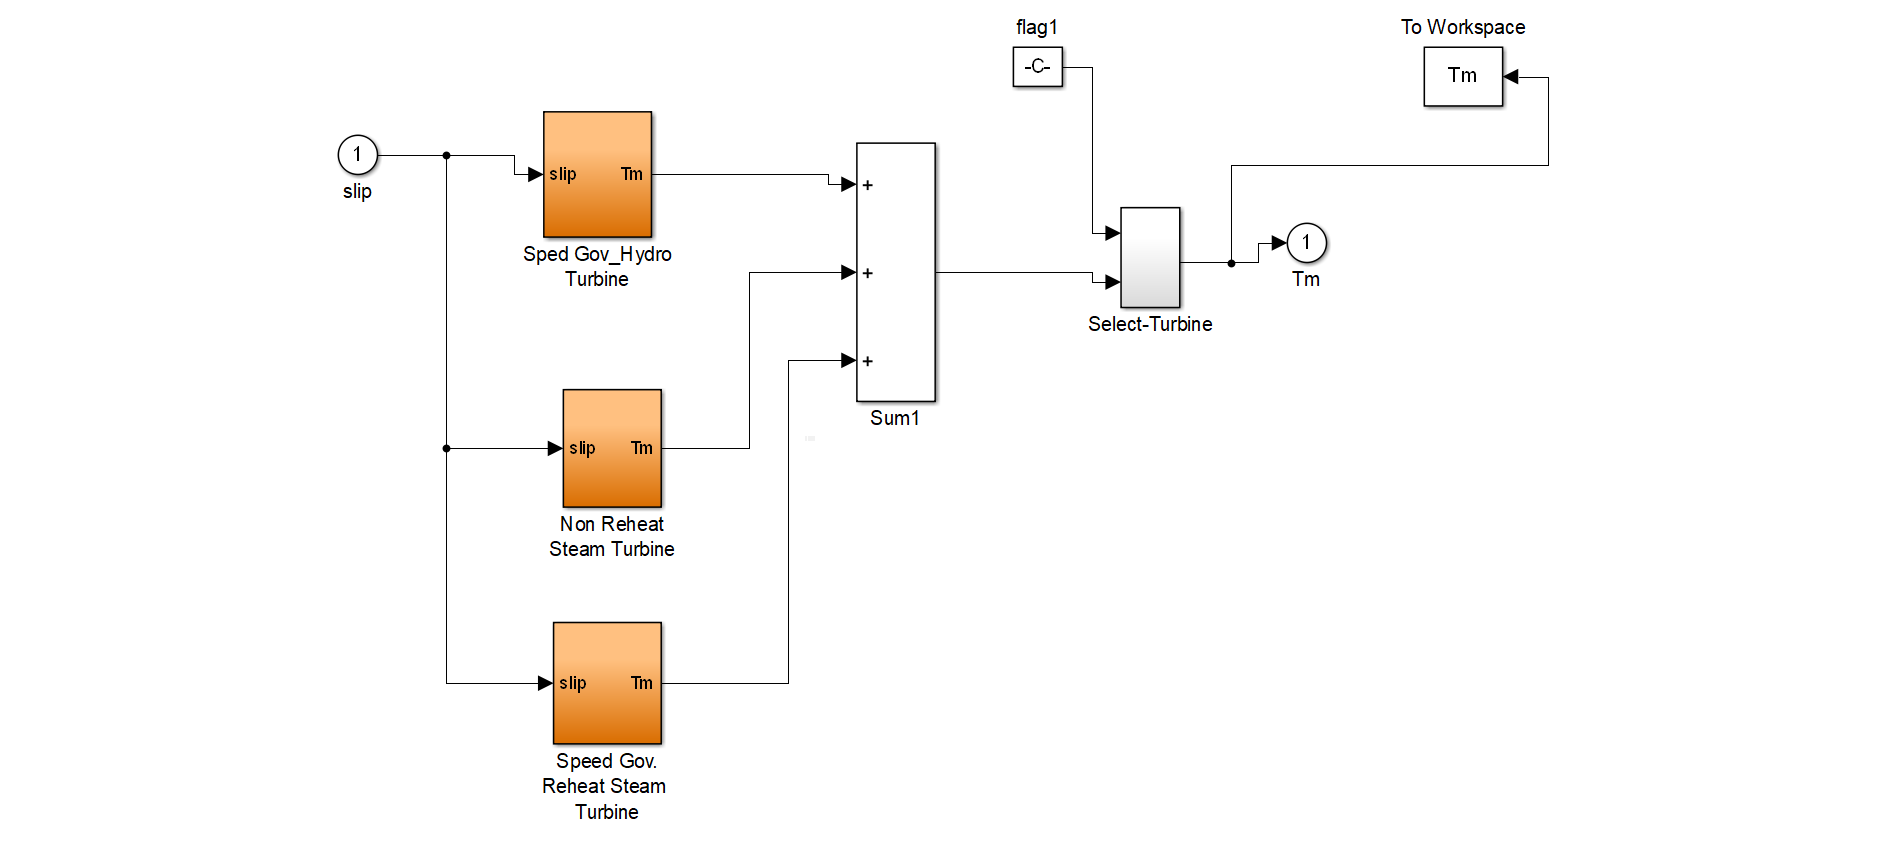
\includegraphics[scale=0.3]{Turbine}
	%\caption{Add your own figures before compiling}
	%\label{some example}
	\end{figure}
	\end{frame} 
	
	
	\begin{frame}
	\frametitle{System Parameters Output in Scope}
	\begin{itemize} \justifying 
	\item 8 System parameters (Generator Angle Deviation, Field EMF, Quadrature Axis Parameter, Direct Axis Parameter, Field Current, Mechanical Torque, Electrical Torque and System Voltage) are loaded to observe the result of transient stability of the system in graphical form.
	\end{itemize}
	\begin{figure}
	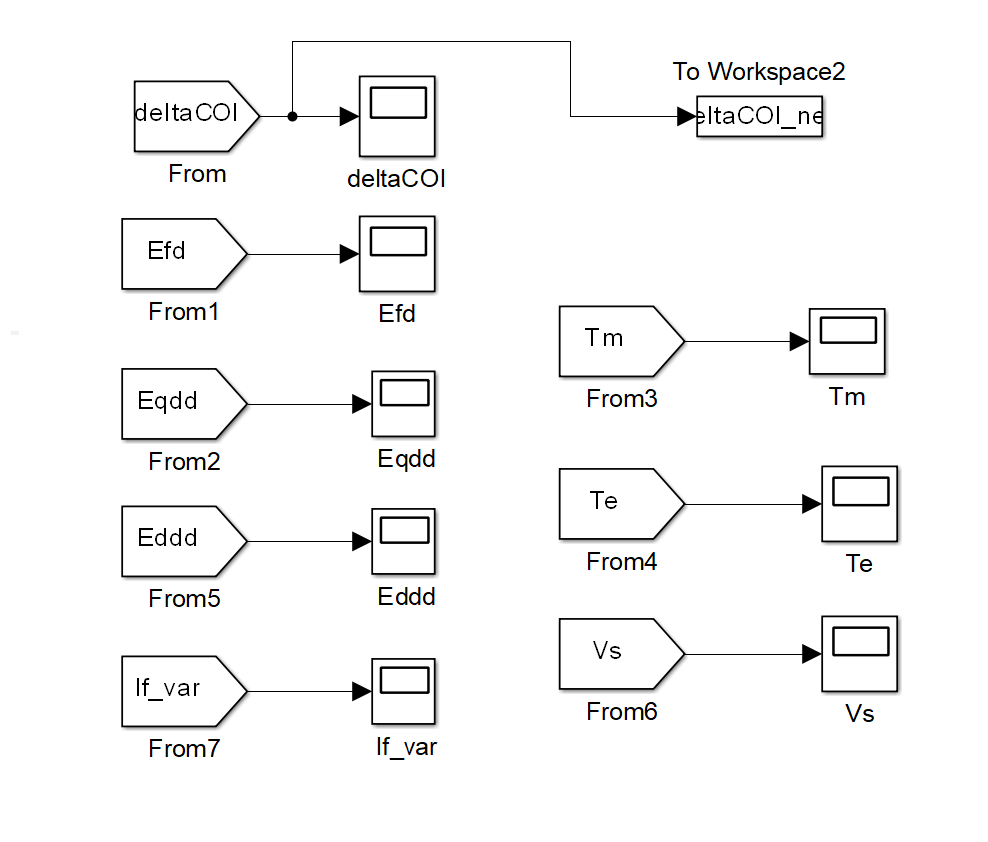
\includegraphics[scale=0.3]{output}
	%\caption{Add your own figures before compiling}
	%\label{some example}
	\end{figure}
	\end{frame} 

	\begin{frame}
	\frametitle{Generator sub-models modified for Indicator Evaluation}
	\begin{itemize} \justifying 
	\item Important part of the Indicator Evaluation is the calculation of rotor angle and and its deviation from center of Inertia (COI).
\item Delta is the rotor angle of generator taken as input here to calculate COI and delta\_COI.
\item COI and delta\_COI are the center of Inertia and Rotor angle deviation from Center of Inertia respectively.

	\end{itemize}
	\begin{figure}
	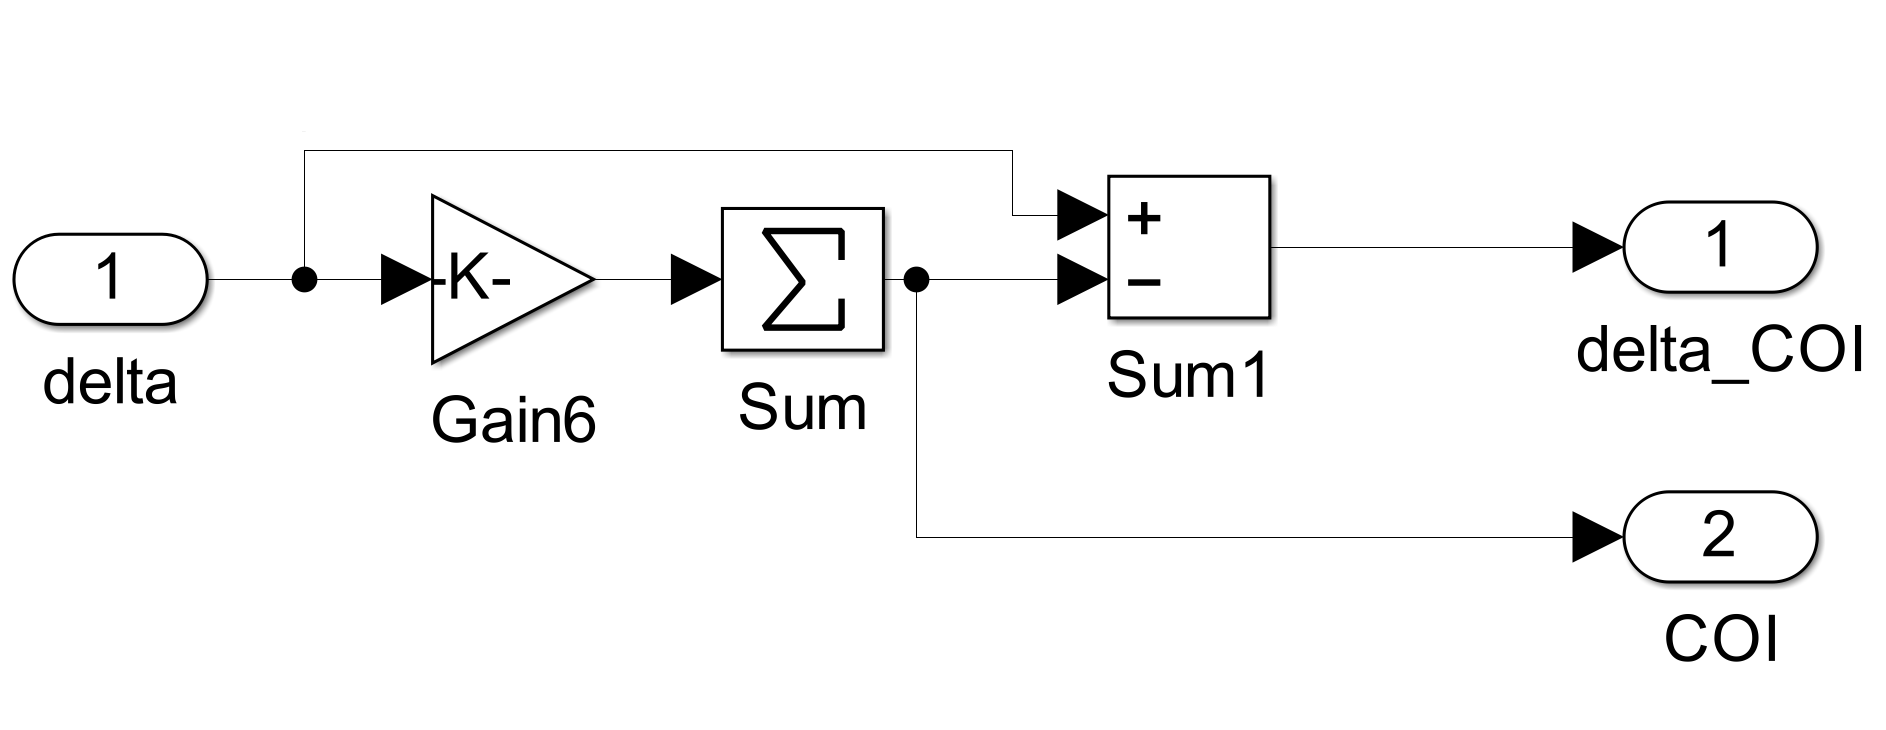
\includegraphics[scale=0.3]{COI Ref}
	%\caption{Add your own figures before compiling}
	%\label{some example}
	\end{figure}
	\end{frame} 
	
	\begin{frame}{Solution Methodology Flowchart}
\begin{figure}[H]
	 \centering
	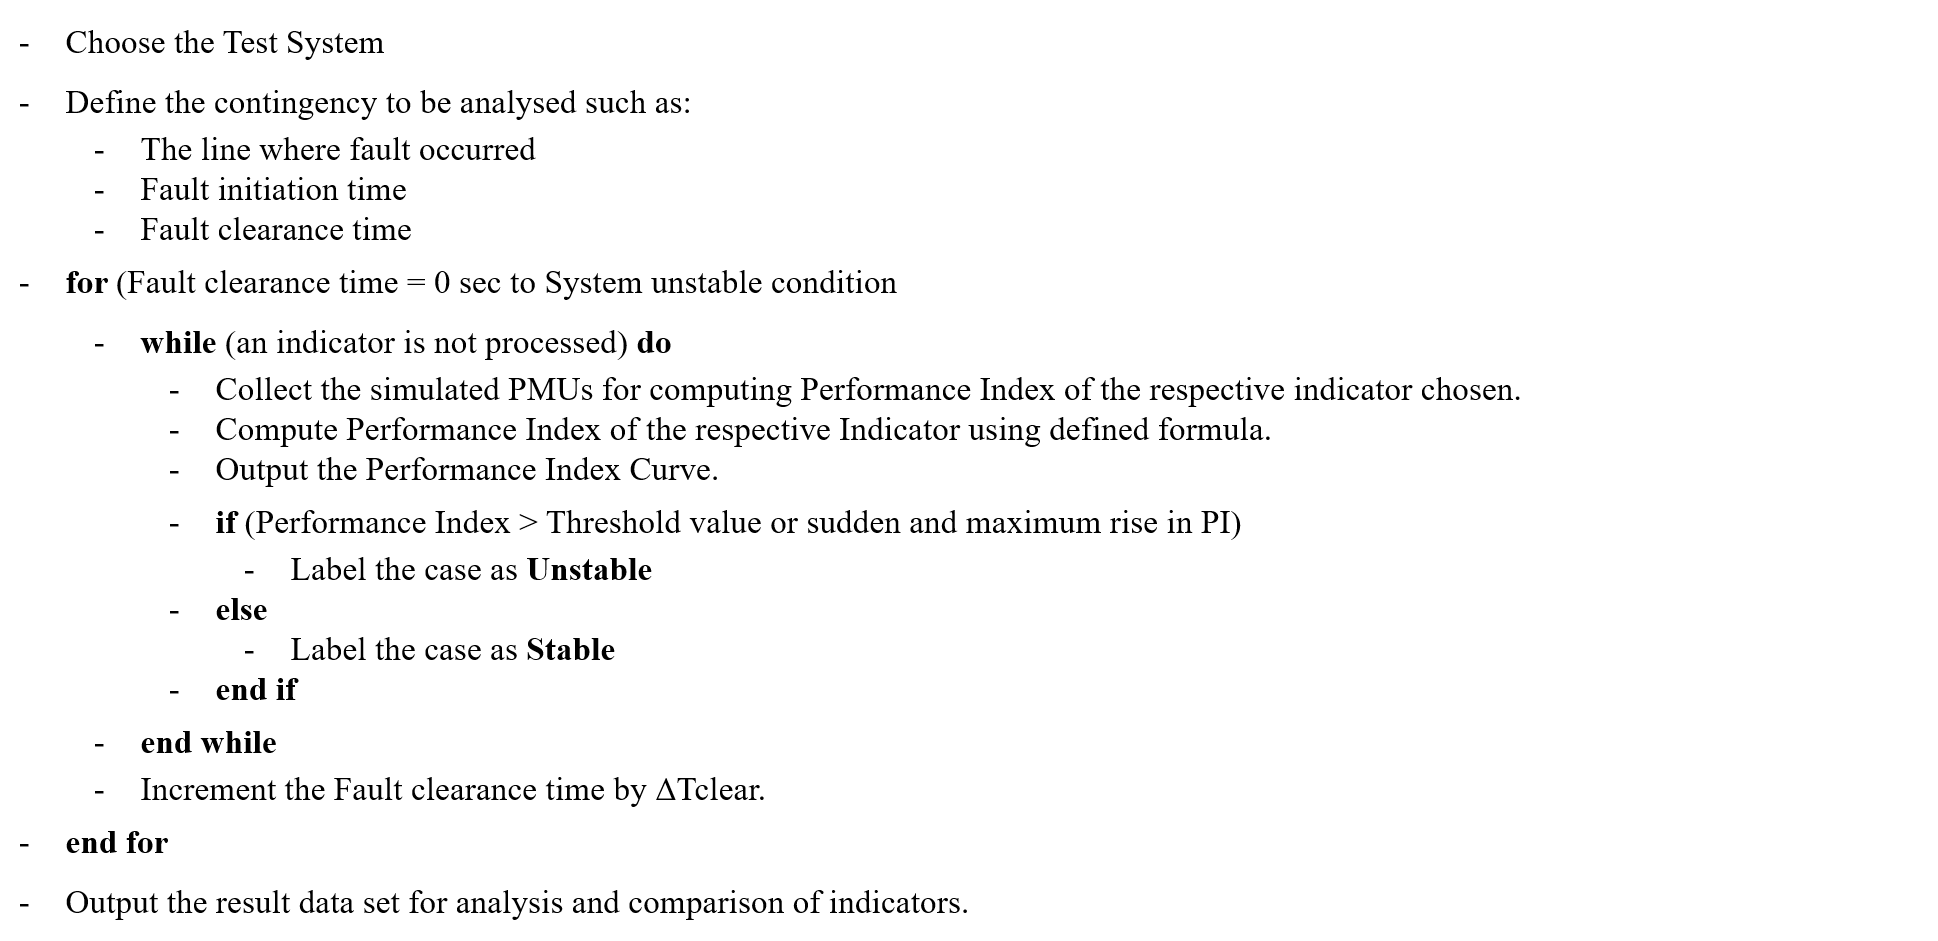
\includegraphics[width=14 cm]{algorithm.png}
	
\end{figure}
\end{frame}

	
%\begin{frame}{Computation of Indicators Algorithm}
%\begin{itemize}
%\item Choose the Test System
%\item Define the contingency to be analysed such as:
%\begin{itemize}
%\item The line where fault occurred
%\item Fault initiation time
%\item Fault clearance time
%\end{itemize}
%\item for (Fault clearance time = 0 sec to System unstable condition
%\begin{itemize}
%\item while (an indicator is not processed) do
%\begin{itemize}
%\item Collect the simulated PMUs for computing Performance Index of the respective indicator chosen.
%\item Compute Performance Index of the respective Indicator using defined formula.
%\item Output the Performance Index Curve.
%\item if (Performance Index > Threshold value or sudden and maximum rise in PI)
%\begin{itemize}
%\item Label the case as Unstable
%\end{itemize}
%\item else
%\begin{itemize}
%\item Label the case as Stable
%\end{itemize}
%\item end if
%\end{itemize}
%\item end while
%\item Increment the Fault clearance time by ΔTclear.
%\end{itemize}
%\item end for
%\item Output the result data set for analysis and comparison of indicators.
%\end{itemize}
%\end{frame}
	
	
	
	
	
	
	
	


\section{Results}

%% Results Introduction-----------------------------------------------------
\begin{frame}{\textbf{Stability Analysis in 10 Bus 4 Generator System}}
\begin{itemize}
\item To illustrate the application of mentioned catastrophic indicators, a practical 10 Bus 4 Generator network system (see fig.) is considered.
\begin{figure}[H]
  \centering
  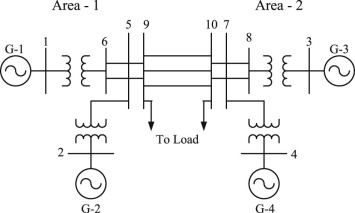
\includegraphics[width=0.3\linewidth]{LD}
  \end{figure}
\item One contingency is considered as follows
\begin{itemize}
\item A base power flow is considered as a steady-state operating point 
\item A three-phase short circuit fault at bus-9 is applied at 0.5 s (Tfault)
\item The fault is cleared in 0.1 s (Tclear) by
opening the line between bus-9 and bus-10 (line contingency).
\end{itemize}
\item So, assuming the fault initiated at 0.5 sec, for different fault clearing
time, the faulted bus is provided for observing the transient stability result from performance of Indicators.
\end{itemize}

\end{frame}

%% Results for Indicator based on Coherency------------------------------
\begin{frame}{\textbf{Results for Indicator based on Coherency}}
Speed Deviation Vs. Time Curve for:-
\begin{figure}
    \centering
\subfloat[No Fault]{
    \includegraphics[width=0.45\textwidth]{Co No fault}}
\subfloat[Tclear = 0.1 sec]{
    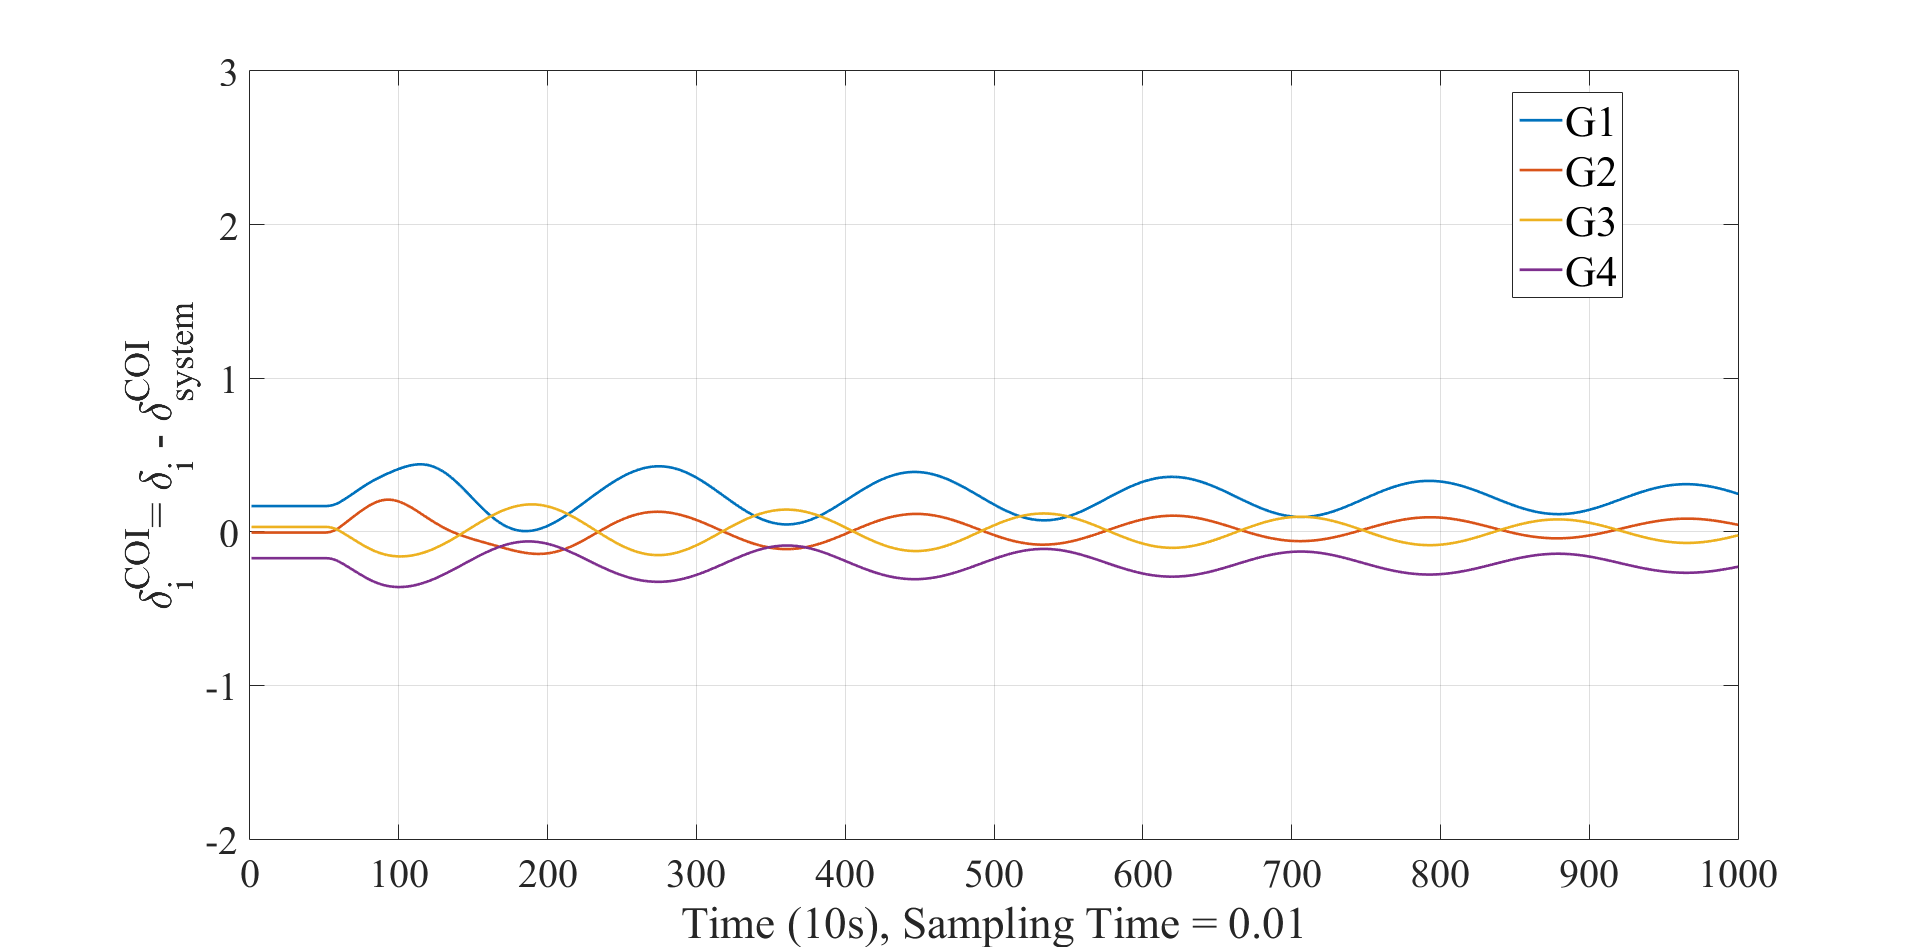
\includegraphics[width=0.45\textwidth]{Co A1}}\\
\subfloat[Tclear = 0.2 sec]{
    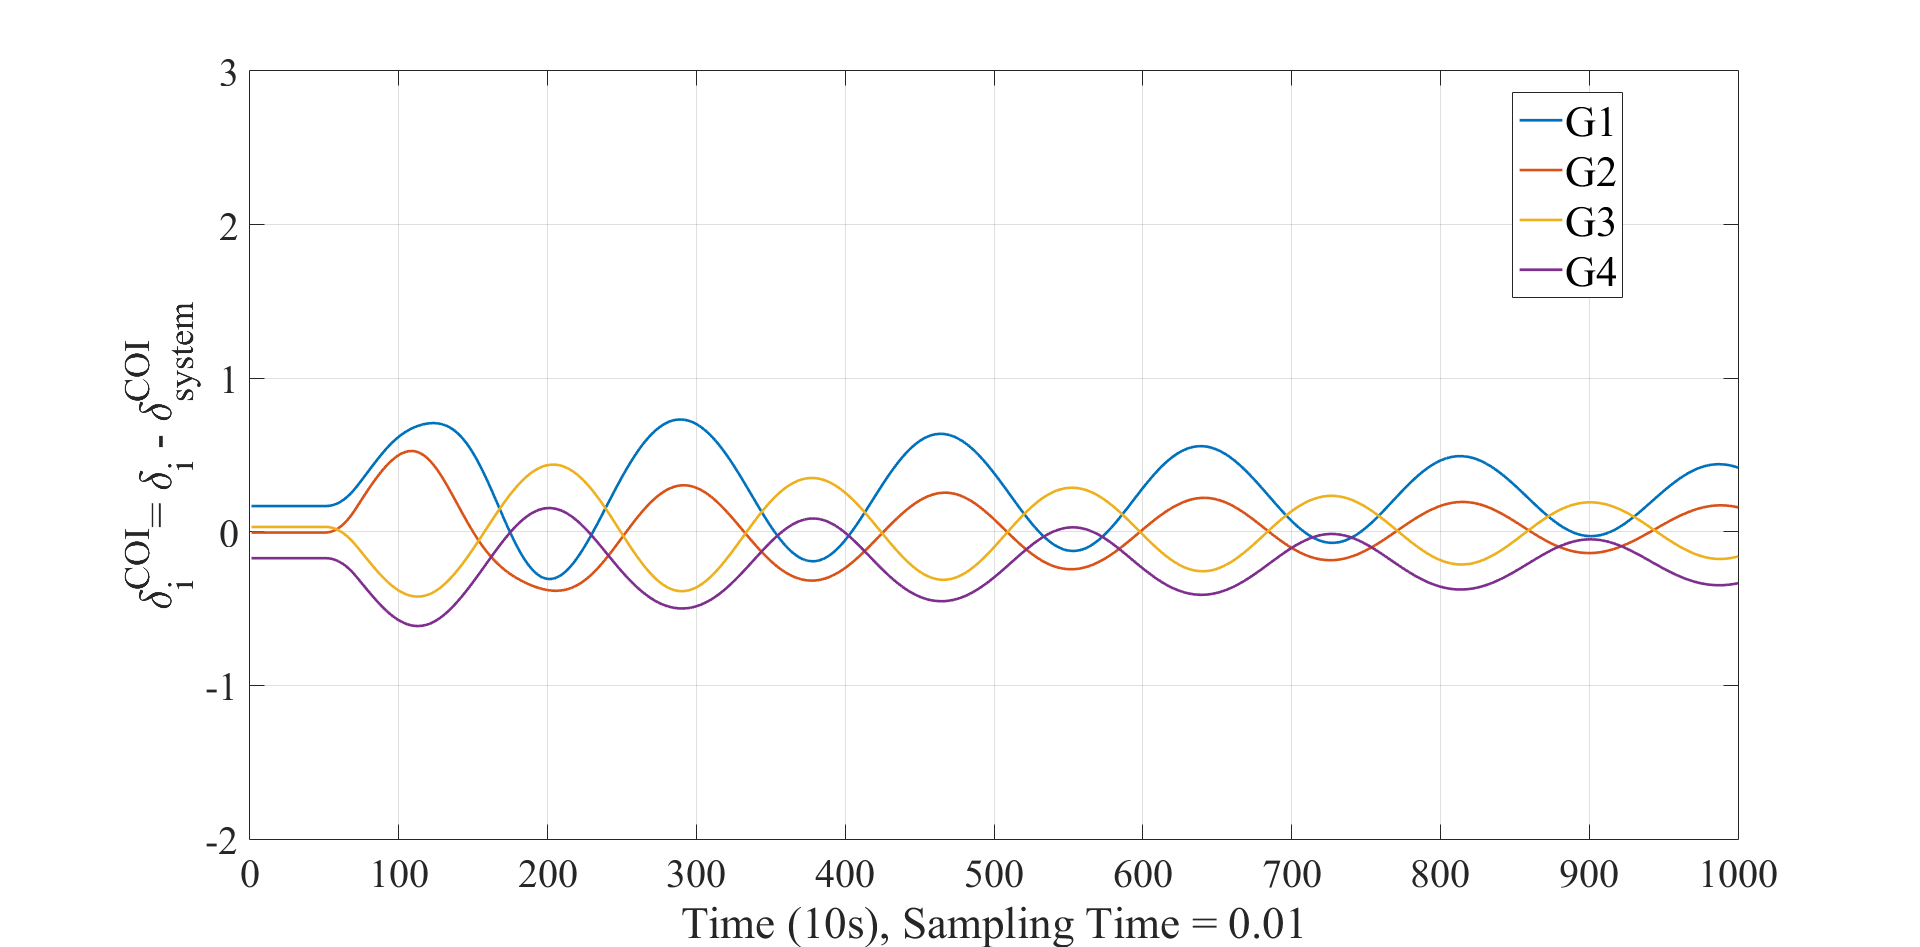
\includegraphics[width=0.45\textwidth]{Co A2}}
\subfloat[Tclear = 0.3 sec]{
    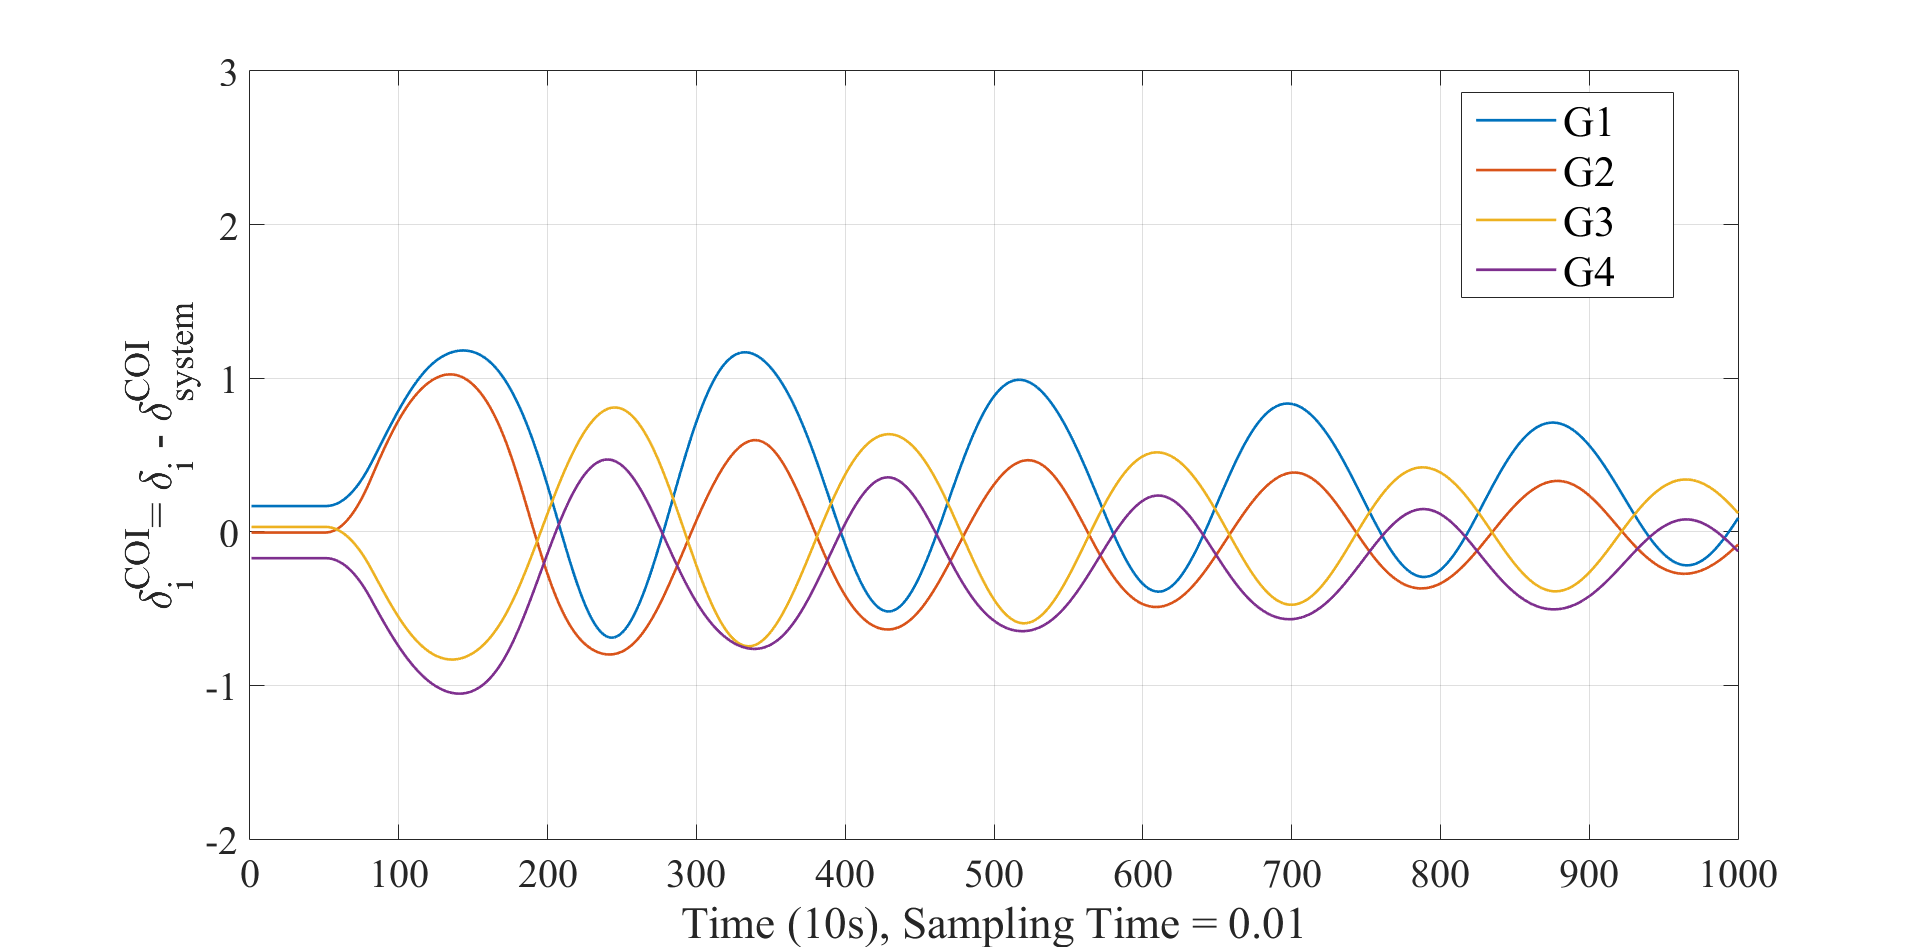
\includegraphics[width=0.45\textwidth]{Co A3}}
\caption{Caption.}
\end{figure}
\end{frame}

\begin{frame}%{\textbf{Results for Indicator based on Coherency} (cont.)}
\begin{figure}
\addtocounter{subfigure}{4}
    \centering
\subfloat[Tclear = 0.4 sec]{
    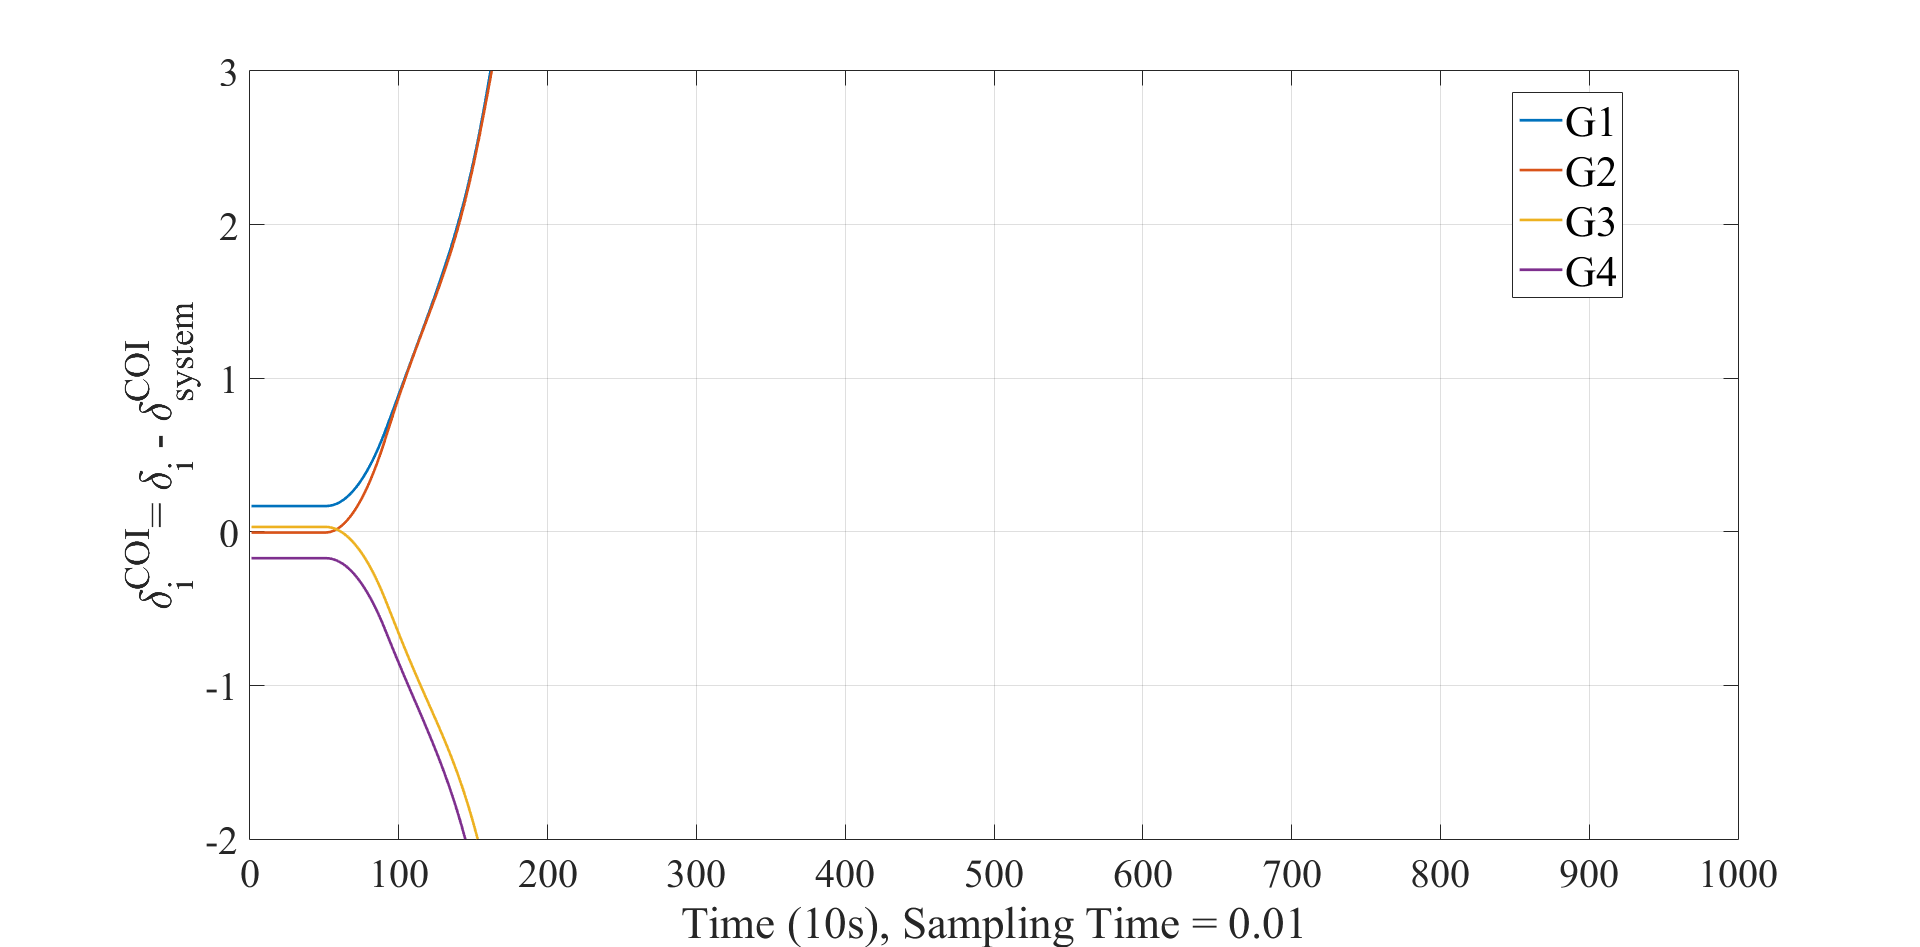
\includegraphics[width=0.45\textwidth]{Co A4}}
%\caption{Caption.}
%\label{fig:caption}
\end{figure}
\begin{table}[H]
\renewcommand{\arraystretch}{1}
\caption{Contingency Analysis using Indicator based on Coherency}
\begin{center}
\begin{tabular}{|c|c|c|}
\hline
 \textbf{Fault Clearing Time} & \textbf{Performance Index} & \textbf{Remarks}  \\ \hline
 No Fault & 1.7262e-10  & Stable \\ \hline
 0.1 sec & 0.4349  & Stable \\ \hline
 0.2 sec & 1.0385  & Stable \\ \hline
 0.3 sec & 1.8697  & Stable \\ \hline
 0.4 sec & 66.9471  & Unstable \\ \hline
\end{tabular}
\end{center}
\end{table}
\end{frame}

%% Results for Indicator based on Transient Energy Conversion--------------
\begin{frame}{\textbf{Results for Indicator based on TEC}\scriptsize{ (Transient Energy Conversion)}}
Transient Energy Vs. Time Curve for:-
\begin{figure}
\setcounter{subfigure}{0}
    \centering
\subfloat[No Fault]{
    \includegraphics[width=0.45\textwidth]{TE No fault}}
\subfloat[Tclear = 0.1 sec]{
    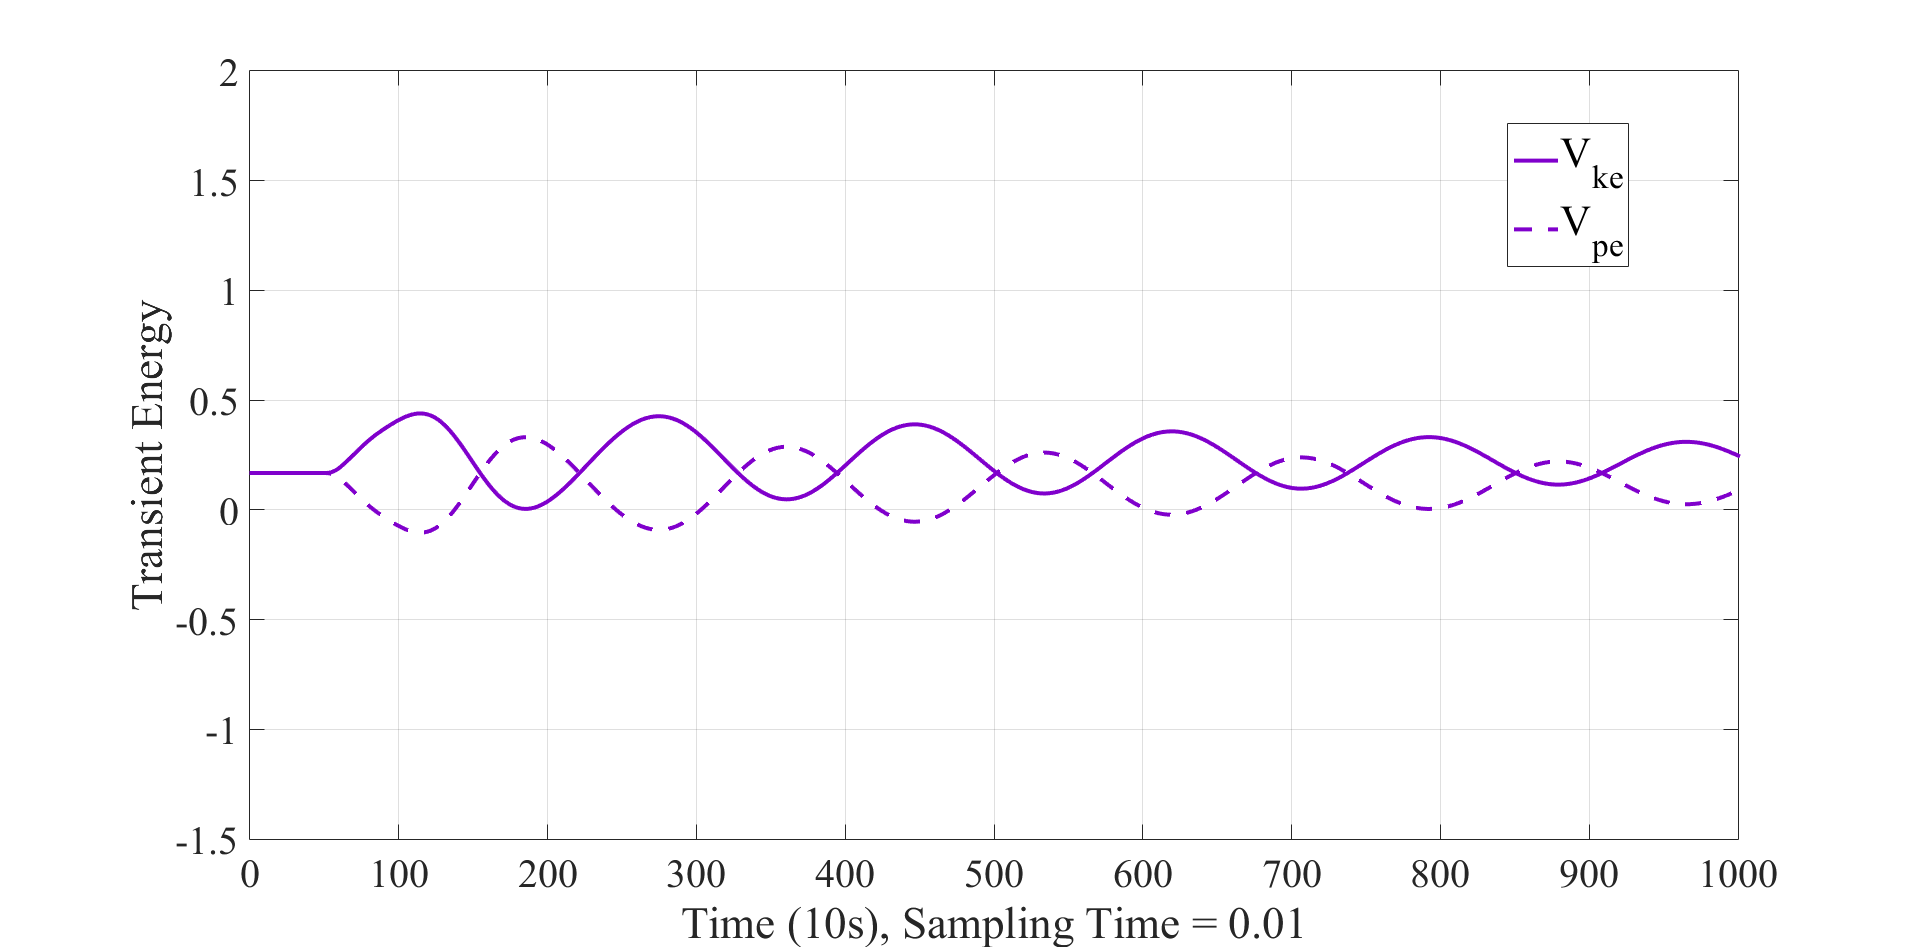
\includegraphics[width=0.45\textwidth]{TE A1}}\\
\subfloat[Tclear = 0.2 sec]{
    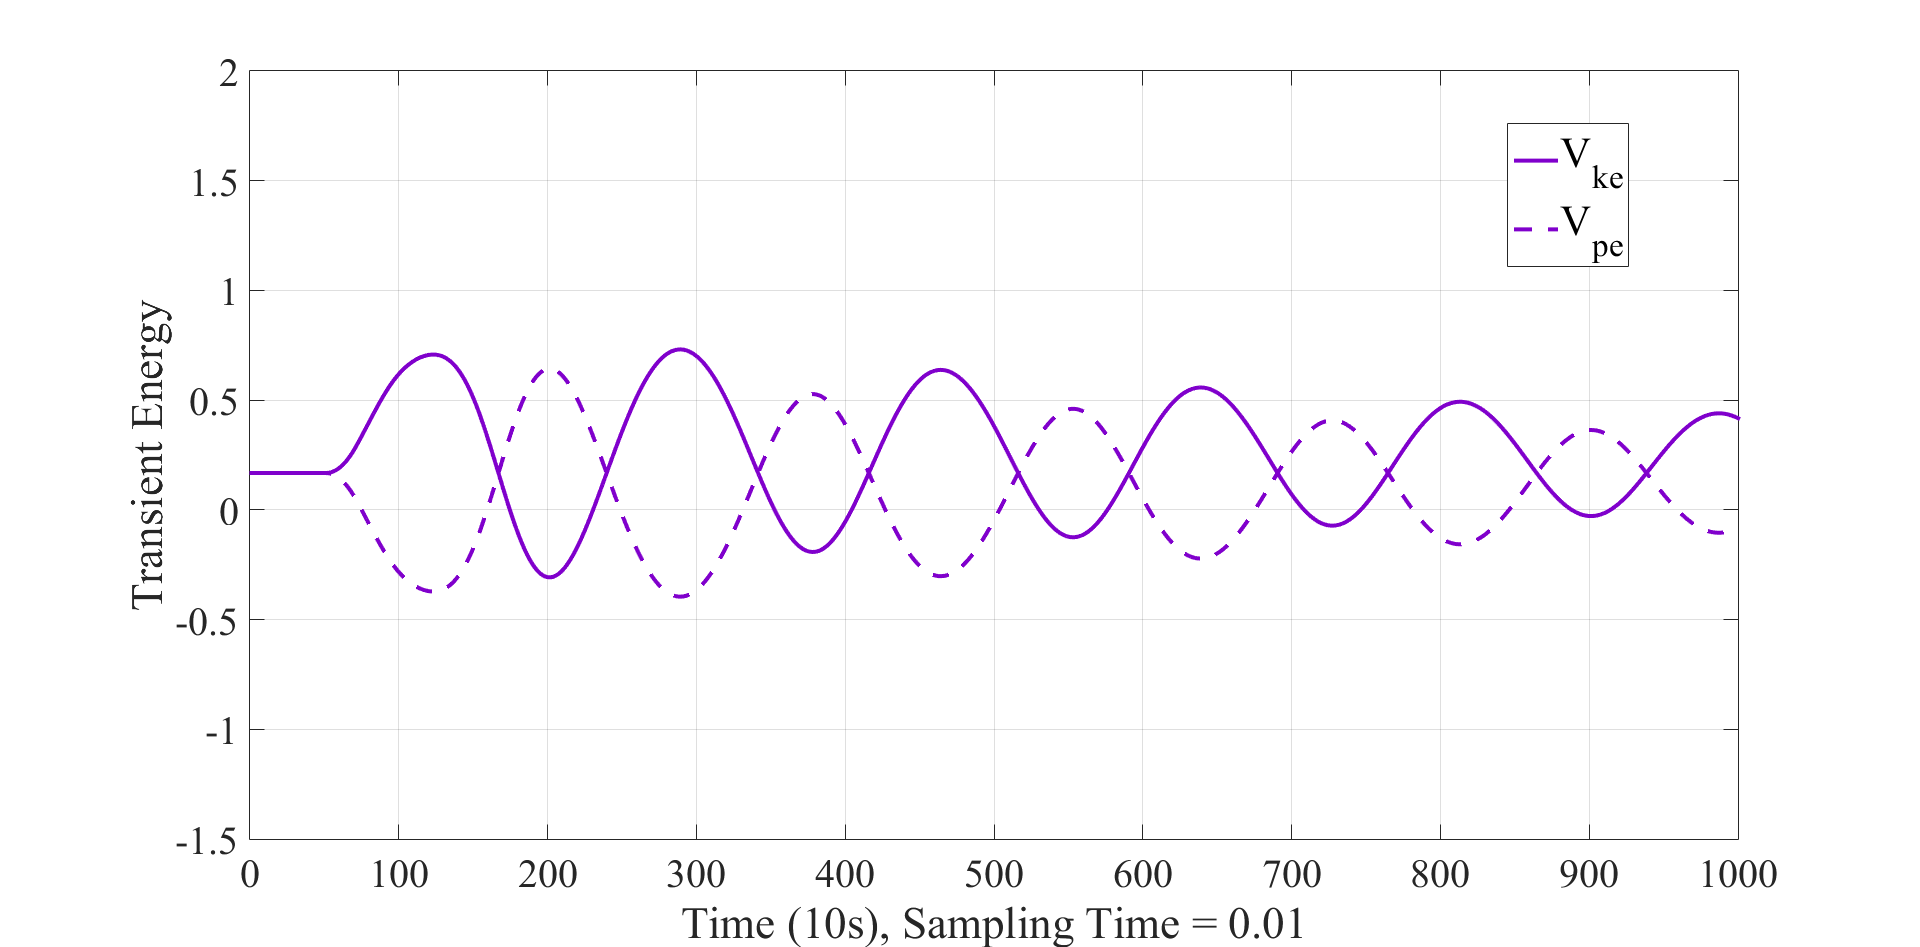
\includegraphics[width=0.45\textwidth]{TE A2}}
\subfloat[Tclear = 0.3 sec]{
    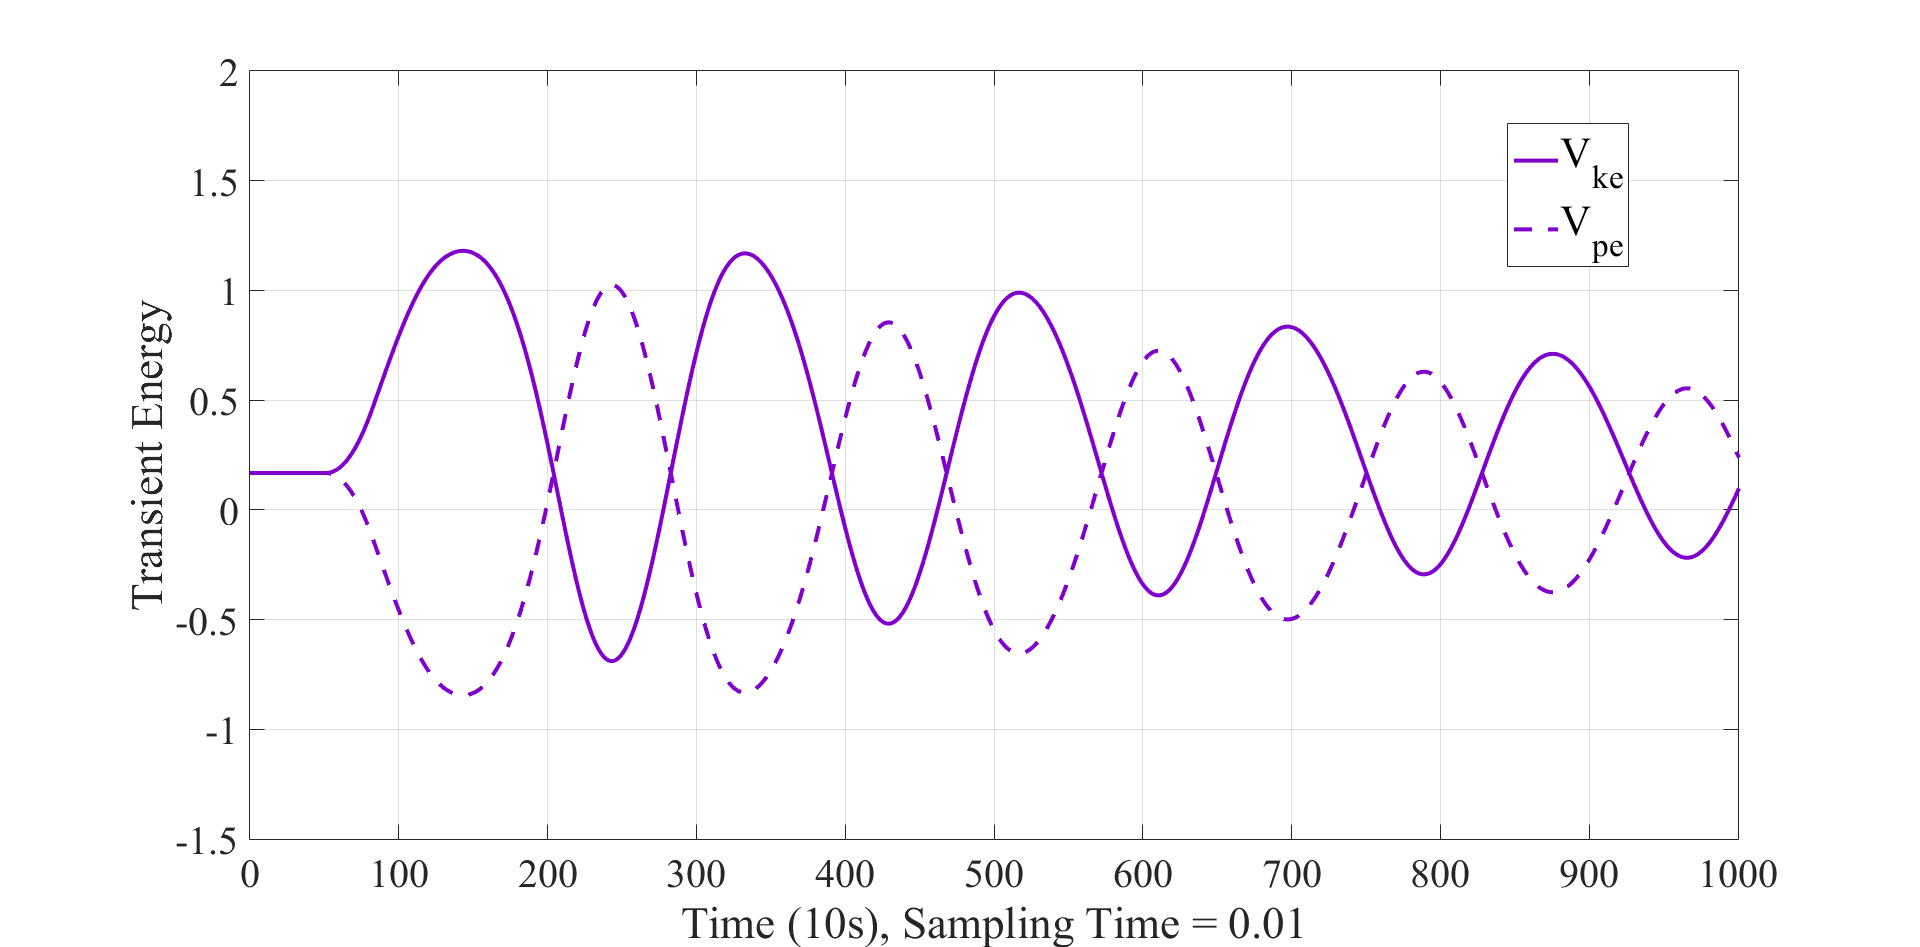
\includegraphics[width=0.45\textwidth]{TE A3}}
\caption{Caption.}
\end{figure}
\end{frame}

\begin{frame}%{\textbf{Results for Indicator based on TEC} (cont.)}
\begin{figure}
\addtocounter{subfigure}{4}
    \centering
\subfloat[Tclear = 0.4 sec]{
    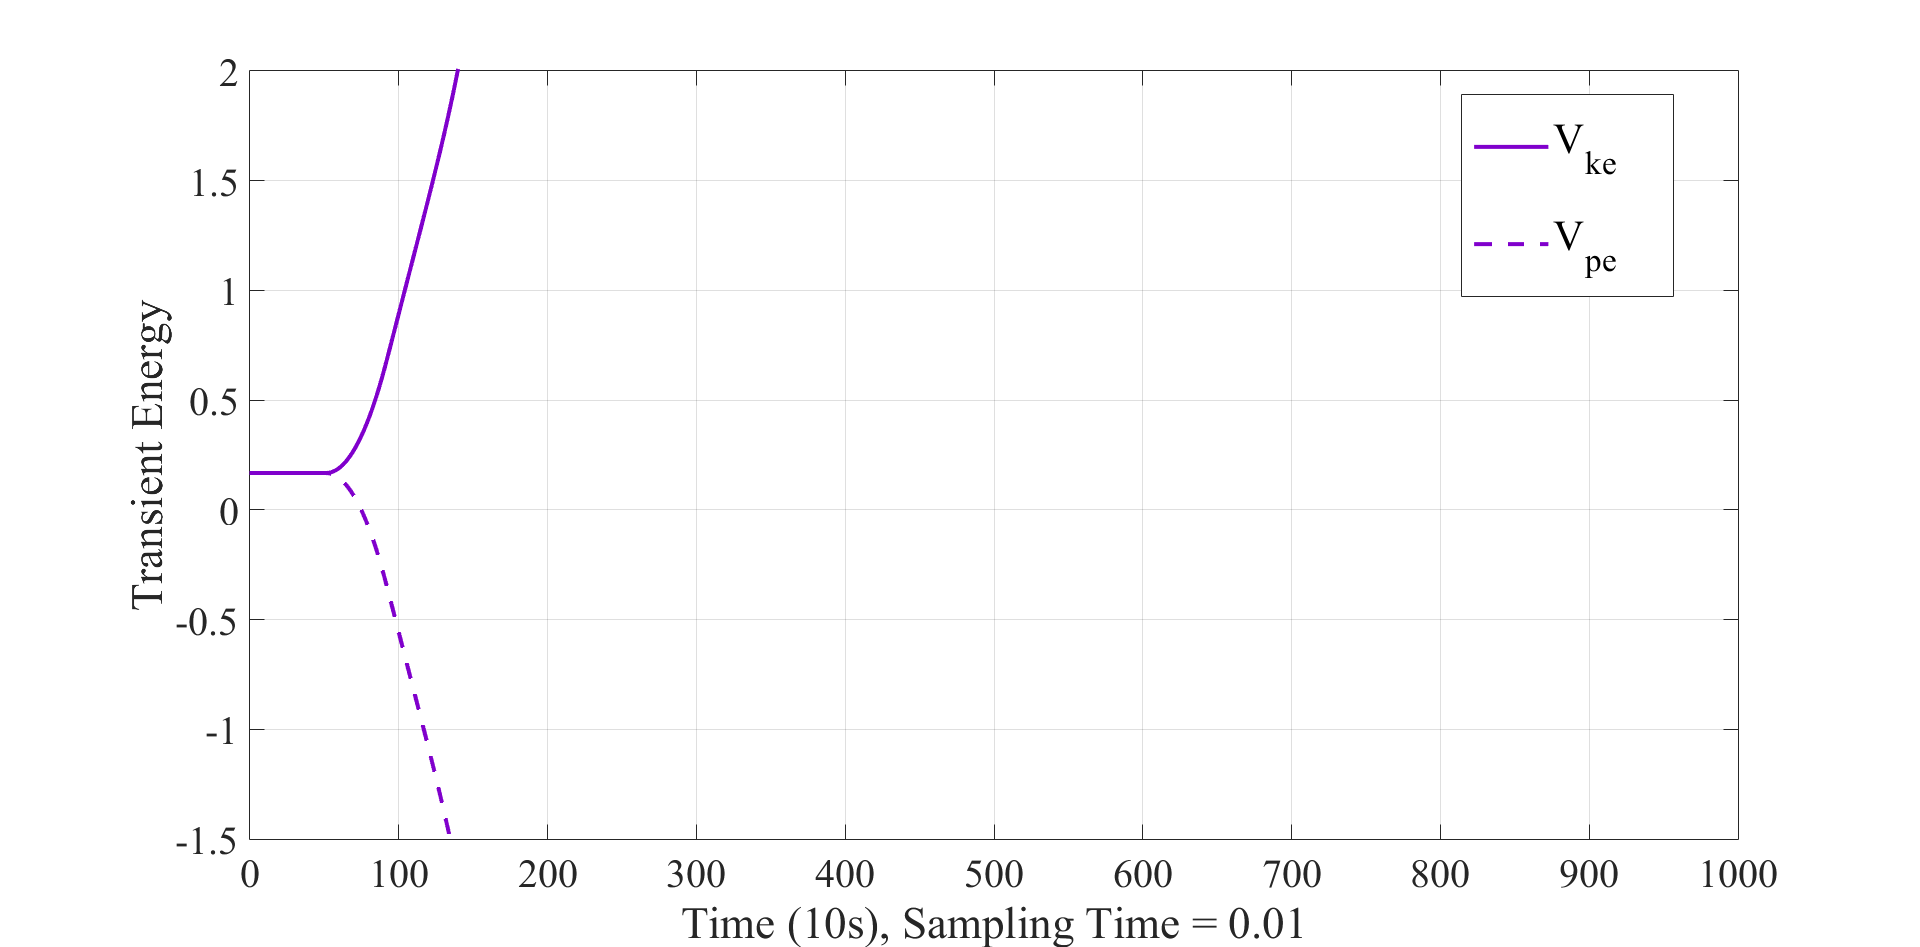
\includegraphics[width=0.45\textwidth]{TE A4}}
%\caption{Caption.}
%\label{fig:caption}
\end{figure}
\begin{table}[H]
\renewcommand{\arraystretch}{1}
\caption{Contingency Analysis using Indicator based on Transient Energy Conversion}
\begin{center}
\begin{tabular}{|c|c|c|}
\hline
 \textbf{Fault Clearing Time} & \textbf{Performance Index} & \textbf{Remarks}  \\ \hline
No Fault & 3.3922e-10  & Stable \\ \hline
 0.1 sec & 0.5432  & Stable \\ \hline
 0.2 sec & 1.1266  & Stable \\ \hline
 0.3 sec & 2.0253  & Stable \\ \hline
 0.4 sec & 133.8941  & Unstable \\ \hline
\end{tabular}
\end{center}
\end{table}
\end{frame}

%% Results for Indicator based on Dot Products (CSA)--------------------
\begin{frame}{\textbf{Results for Indicator based on Dot Products: Contingency Severity Assessment (CSA)}}

\begin{figure}
    \centering
    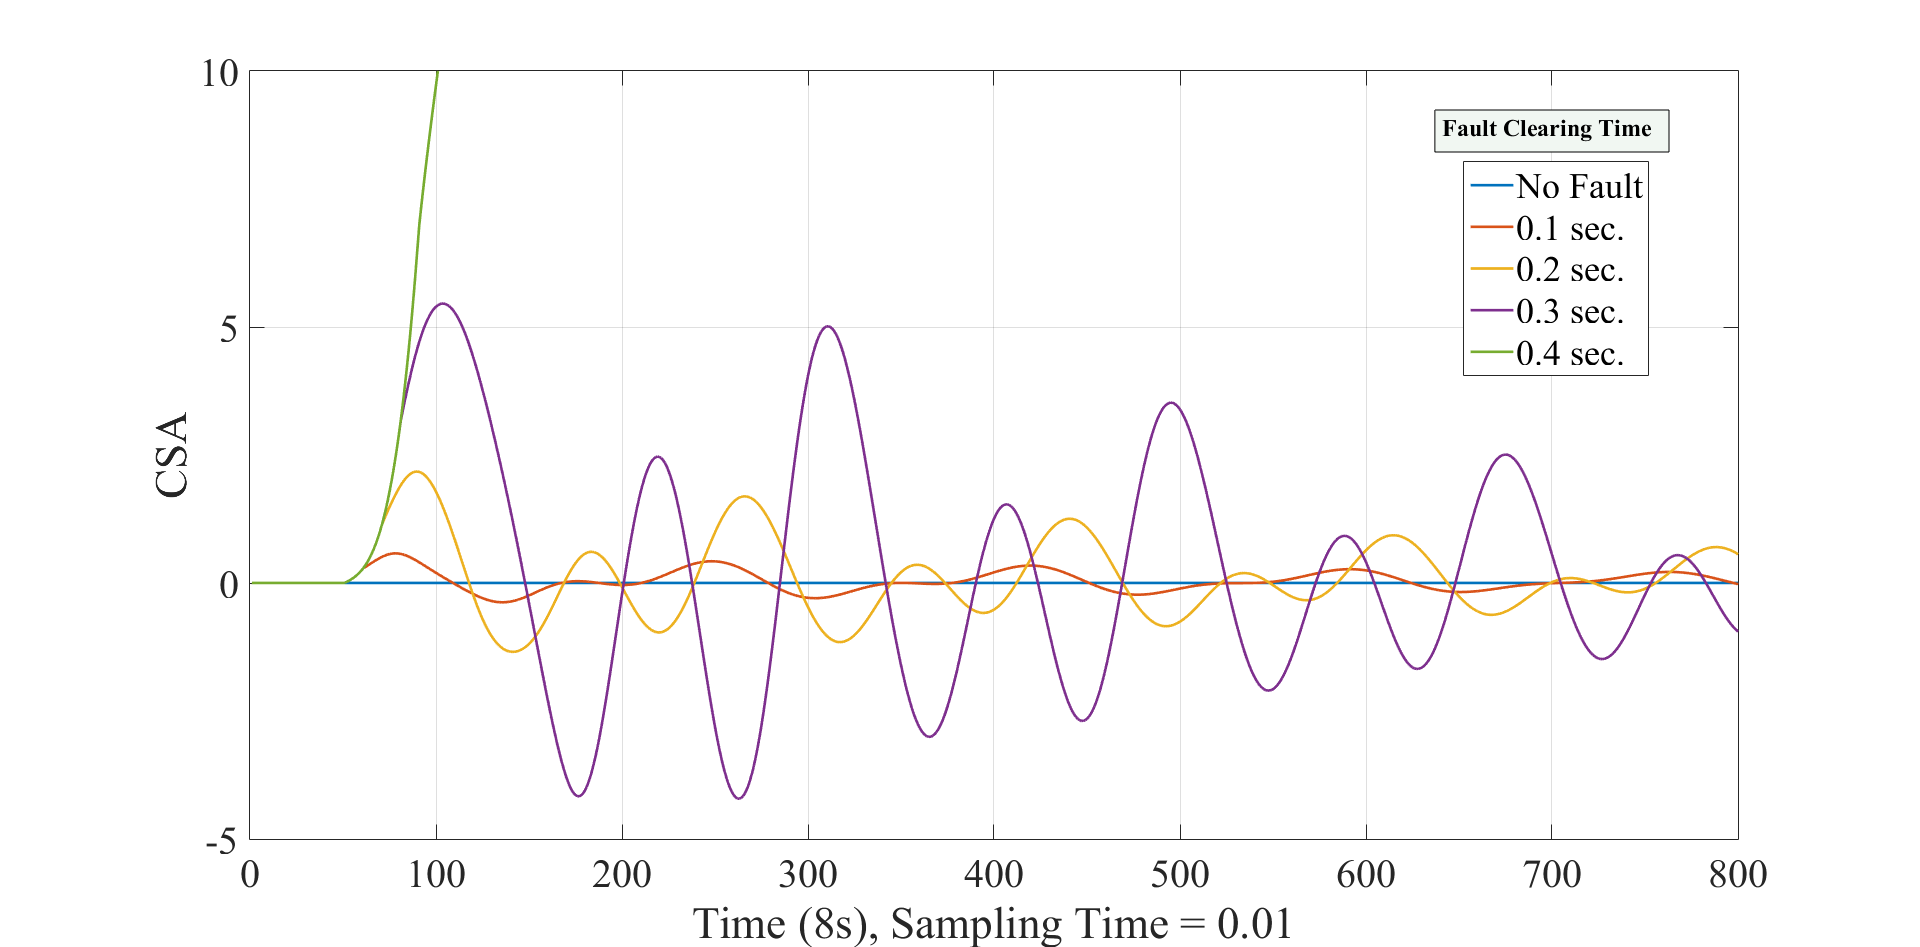
\includegraphics[width=0.9\textwidth]{CSA}
\caption{Contingency Severity Assessment Vs. Time Curve for different Tclear}
\end{figure}
\end{frame}

\begin{frame}%{\textbf{Results for Indicator based on Dot Products: Contingency Severity Assessment (CSA)} (cont.)}
\begin{table}[H]
\renewcommand{\arraystretch}{1}
\caption{Contingency Analysis using Indicator based on Dot Products: Contingency Severity Assessment (CSA)}
\begin{center}
\begin{tabular}{|c|c|c|}
\hline
 \textbf{Fault Clearing Time} & \textbf{Performance Index} & \textbf{Remarks}  \\ \hline
 No Fault & 1.5902e-10  & Stable \\ \hline
 0.1 sec & 0.9557  & Stable \\ \hline
 0.2 sec & 3.5214  & Stable \\ \hline
 0.3 sec & 9.6711  & Stable \\ \hline
 0.4 sec & 2.4770e+03  & Unstable \\ \hline
\end{tabular}
\end{center}
\end{table}
\end{frame}

%% Results for Indicator based on Wide Area Severity Index (WASI)--
\begin{frame}{\textbf{Results for Indicator based on Wide Area Severity Index (WASI)}}
\begin{figure}
    \centering
    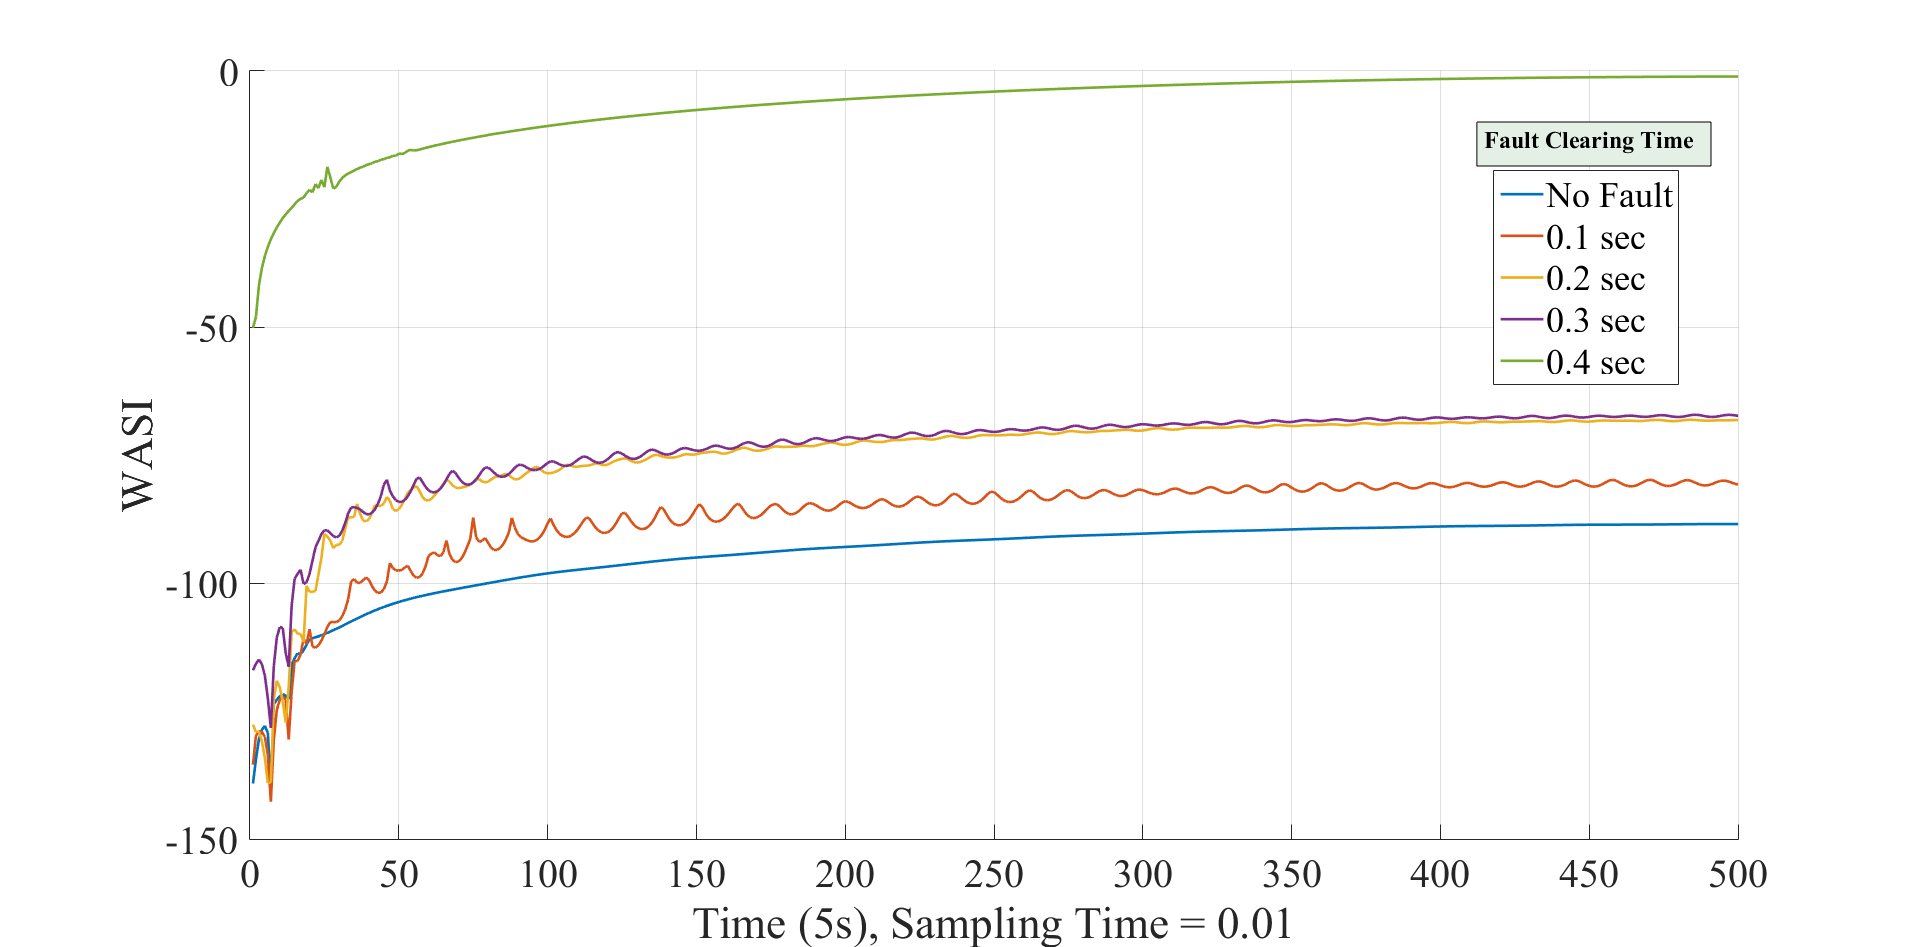
\includegraphics[width=0.9\textwidth]{WASIcurve}
\caption{Wide Area Severity Index Vs. Time Curve for different Tclear}
\end{figure}
\end{frame}

\begin{frame}%{\textbf{Results for Indicator based on Dot Products: Contingency Severity Assessment (CSA)} (cont.)}
\begin{table}[H]
\renewcommand{\arraystretch}{1}
\caption{Contingency Analysis using Indicator based on Wide Area Severity Index (WASI)}
\begin{center}
\begin{tabular}{|c|c|c|}
\hline
 \textbf{Fault Clearing Time} & \textbf{Performance Index} & \textbf{Remarks}  \\ \hline
No Fault & -88.4891  & Stable \\ \hline
 0.1 sec & -80.7781  & Stable \\ \hline
 0.2 sec & -68.1678  & Stable \\ \hline
 0.3 sec & -67.3590  & Stable \\ \hline
 0.4 sec & -1.0775  & Unstable \\ \hline
\end{tabular}
\end{center}
\end{table}
\end{frame}

%% Results for Indicator based on Inter-area Stability Prediction Index----
\begin{frame}{\textbf{Results for Indicator based on Inter-area Stability Prediction Index}}
\begin{table}[H]
\renewcommand{\arraystretch}{1}
\caption{Contingency Analysis using Indicator based on Inter-area Stability Prediction Index (ISPI)}
\begin{center}
\begin{tabular}{|c|c|c|}
\hline
 \textbf{Fault Clearing Time} & \textbf{ISPI} & \textbf{Remarks}  \\ \hline
 No Fault & 0.0000  & Stable \\ \hline
 0.1 sec & 3.1537  & Stable \\ \hline
 0.2 sec & 11.6207  & Stable \\ \hline
 0.3 sec & 31.9145  & Stable \\ \hline
 0.4 sec & 82.5676  & Unstable \\ \hline
 0.5 sec & 92.5350  & Unstable \\ \hline
\end{tabular}
\end{center}
\end{table}
\end{frame}

\begin{frame}
\begin{figure}
    \centering
    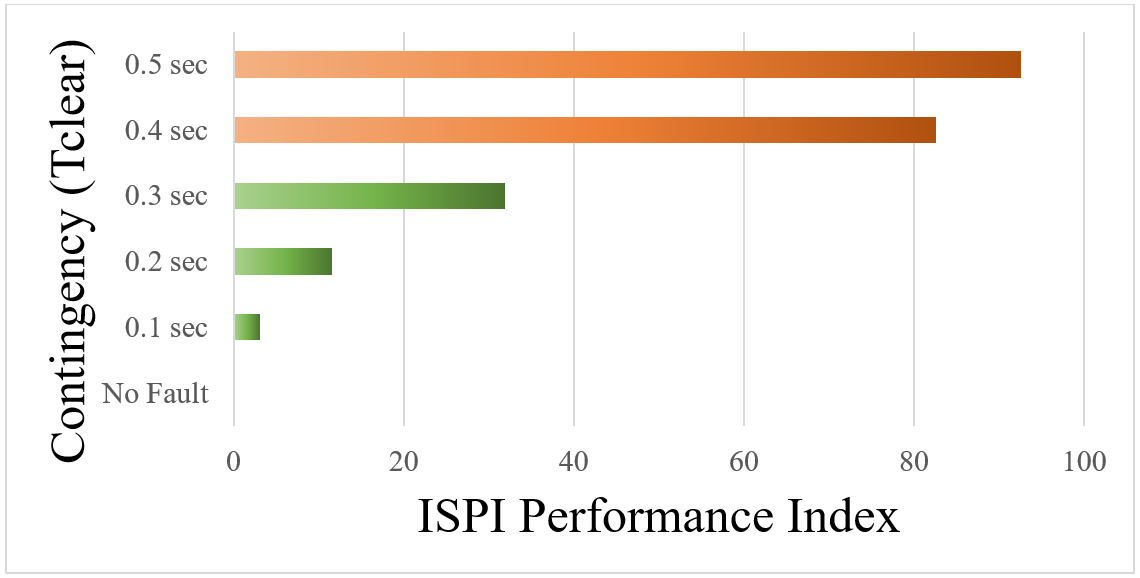
\includegraphics[width=0.9\textwidth]{ISPI Bar graph}
\caption{Graphical Representation of Inter-area Stability Prediction Index (ISPI)}
\end{figure}
\end{frame}

	\begin{frame}{Stability Analysis in Different Contingencies
}
\begin{figure}[H]
	 \centering
	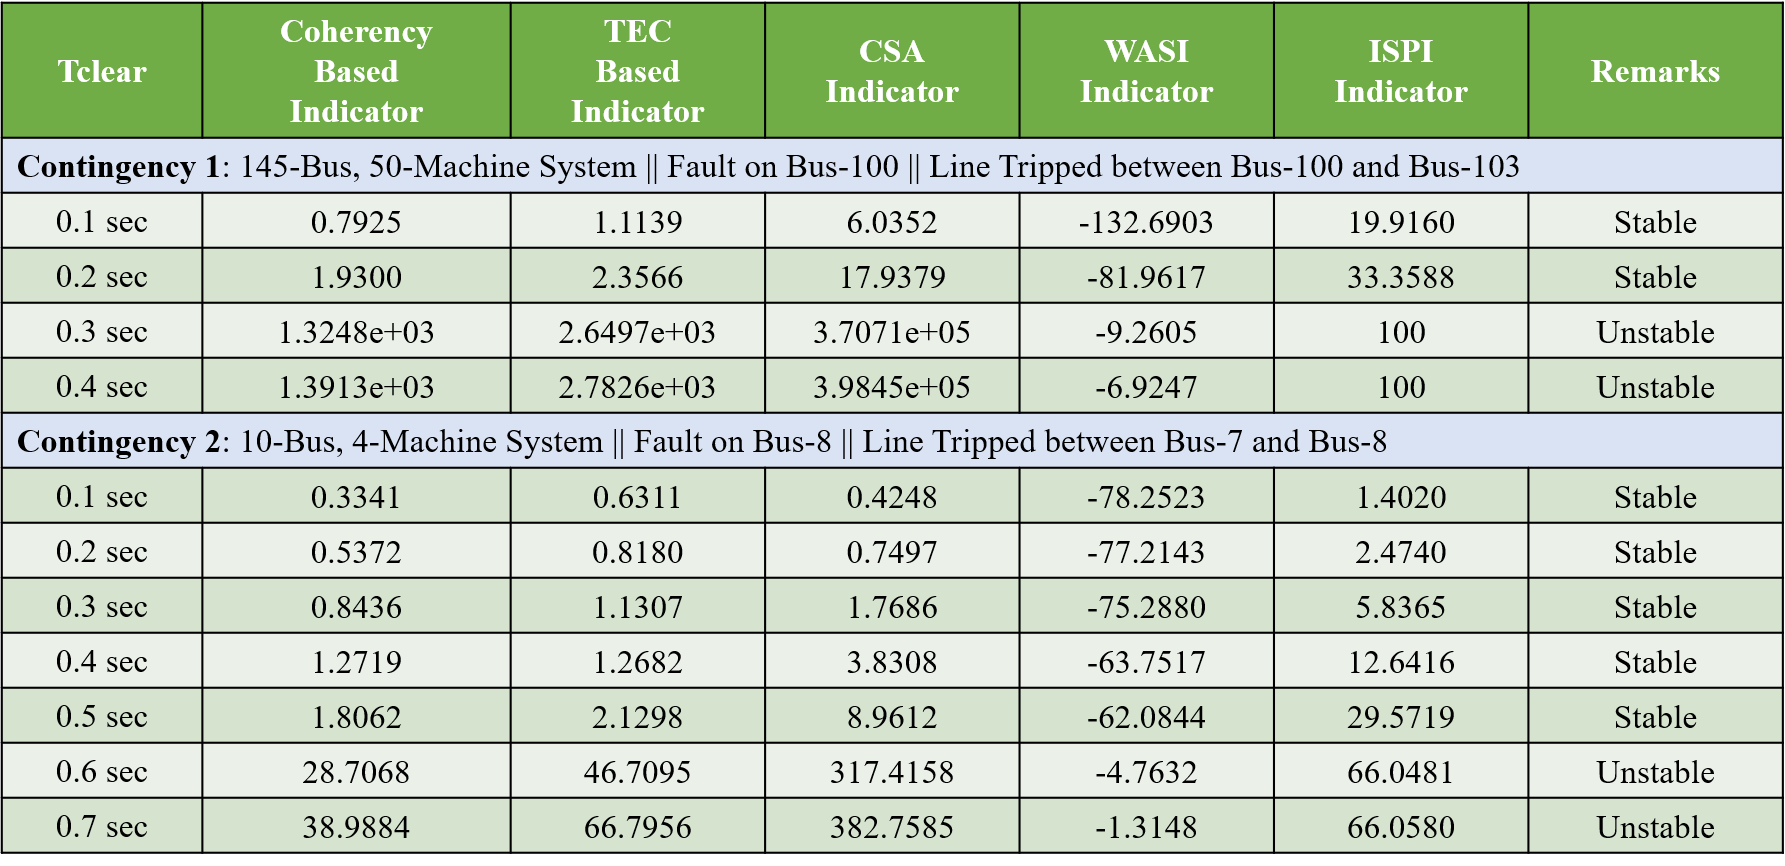
\includegraphics[width=12 cm]{other contingencies.png}
	
\end{figure}
\end{frame}

%% Results Discussion-----------------------------------------------------
\begin{frame}{\textbf{Results Discussion}}
\begin{itemize} \justifying 
	\item As sudden and large deviation in the curve are considered for analyzing the system behavior, i.e. Stable or Unstable, so the clear margin decides the strength of Indicator.
\item Indicator based on coherency is very much simple and depends only on one parameter i.e.  Rotor angle coherency,  which is both advantage and disadvantage to the system. Its PI changes from 1.8697 to 66.9471 in $\Delta Tclear$ = 0.1 sec.
\item Indicator based on Transient energy conversion performance index changed from 2.0253 to 133.8941 in $\Delta Tclear$ = 0.1 sec., the margin quite large from indicator based on coherency.
\item Indicator base on dot products gives a fast, coarse and conservative ranking of the contingencies. Looking at its performance index the margin is quite large compared to both the above indicators, as its PI changes from 9.6711 to 2477  for $\Delta Tclear$ = 0.1 sec.

\end{itemize}
\end{frame}

\begin{frame}{\textbf{Results Discussion (cont.)}}
\begin{itemize} \justifying
\item WASI don’t show large margin in comparison to other but it can cover the exponentially rising high power signal energy.
\item ISPI standardizes the system performance in the range 100\%, by which the large system values converted to ISPI clearly differentiate between stable and unstable along with Normal, Alert and Alarming situation.

\end{itemize}
\end{frame}

\begin{frame}{\textbf{Conclusion}}
\begin{itemize} \justifying
\item After disturbance has been addressed, these indicators are focused on coherency, transient energy conversion between kinetic and potential energy, dot products, and generator coupling parameters.
\item These indices are quick to calculate because they don’t require a lengthy simulation to determine if a situation is stable or unstable as well as precise because they have a high probability of capturing all unstable circumstances.
\item These indices have been examined on a variety of test systems in the background while developing project including the discussed contingencies, and the findings indicate that the result provided by each of the indicator is correct and match to the original data. 
\item The possibility of mis-detection is zero till now, so this could be useful in future contingency screening.
\item And it is well known that some indices work better than others for particular power systems and that combinations of indices usually work better than a single index.

\end{itemize}
\end{frame}

\begin{frame}{\textbf{Future Scope
}}
\begin{itemize} \justifying
\item The catastrophic indicators have been analyzed through a single method i.e. observing sudden and large deviation in the curve to analyze the system behavior in my paper. 
\item But there is need to define Threshold values for each indicator to observe the system behavior after fault. So, finding threshold values through any type of optimization method or any other makes this Indicator Evaluation a complete process. 
\item Execution of these indicators in parallel with a better computational performance can be achieved by developing an online implementation framework. The framework can be developed either by a high-performance computing (HPC) or by a parallel processing architecture.


\end{itemize}
\end{frame}

\begin{frame}{\textbf{Selected References}}
\begin{itemize} \justifying
\item Zimmerman, R.D., Murillo-Sánchez, C.E. and Thomas, R.J., 2010. MATPOWER: Steady-state operations, planning, and analysis tools for power systems research and education. IEEE Transactions on power systems, 26(1), pp.12-19.
\item Ravikumar, G. and Khaparde, S.A., 2016. Taxonomy of PMU data based catastrophic indicators for power system stability assessment. IEEE Systems Journal, 12(1), pp.452-464.
\item Ravikumar, G., 2016. MATTRANS: a MATLAB power system transient stability simulation package. url: https://github. com/gelliravi/MatTrans.
\item Fu, C. and Bose, A., 1999. Contingency ranking based on severity indices in dynamic security analysis. IEEE Transactions on power systems, 14(3), pp.980-985.


\end{itemize}
\end{frame}

\begin{frame}{\textbf{Selected References(cont.)}}
\begin{itemize} \justifying
\item Gomez, O. and Rios, M.A., 2012, January. Inter-area stability prediction index based on phasorial measurement. In 2012 IEEE PES Innovative Smart Grid Technologies (ISGT) (pp. 1-8). IEEE.
\item Sobbouhi, A.R. and Vahedi, A., 2020. Online synchronous generator out-of-step prediction by ellipse fitting on acceleration power–Speed deviation curve. International Journal of Electrical Power \&  Energy Systems, 119, p.105965.
\item Sobbouhi, A.R. and Vahedi, A., 2021. Transient stability prediction of power system; a review on methods, classification and considerations. Electric Power Systems Research, 190, p.106853.


\end{itemize}
\end{frame}







\end{document}
